\documentclass[twocolumn]{article}
\usepackage{titling}
\usepackage{lipsum}
\usepackage{hyperref}
\usepackage{indentfirst}
\usepackage{graphicx}
\usepackage{float}
\usepackage{amsmath}
\usepackage{mathtools}
\usepackage{booktabs}
\usepackage{tabularx}
\usepackage{siunitx}
\usepackage{tabularx}
\usepackage{geometry}
\usepackage{enumitem}
\usepackage[backend=bibtex, style=authoryear, sorting=none]{biblatex}
\addbibresource{references.bib}



\setlength{\parindent}{2em}

\title{Predicting Individual Income through Household Demographic Statistics: A Data-driven Approach}
\author{
	Hsun-Hao Chang\thanks{leo20020529@gmail.com, Student ID: 110502528}\and 
	Po-Shen Chen\thanks{boson13579@gmail.com, Student ID: 110502529}\and 
	Hung-Yi Hsu\thanks{110502009@cc.ncu.edu.tw, Student ID: 110502009}\and 
	Chun-Yu Chen\thanks{fancy0.0turkey@gmail.com, Student ID: 110502534}
}
\date{\today}

\begin{document}
\begin{titlepage}
    \maketitle
    \thispagestyle{empty}
\end{titlepage}

\begin{abstract}
This research investigates and compares the performance of multiple machine learning models on the task of predicting individual income using data from the Household Income Survey in the Republic of China. The dataset includes personal attributes such as YEAR, REL, SEX, AGE, EDU, IND, OCC, WKCLASS, WORK, IMR, WORKPLACE, MRG, which are utilized to predict individual income. A comprehensive set of machine learning models, including but not limited to Extremely Trees Regressor, Random Forest Regressor, Bagging Regressor, HistGradientBoosting Regressor, GradientBoosting Regressor, Decision Tree Regressor, Support Vector Regressor (SVR), NuSVR, Extremely Tree Regressor, MLP Regressor, Linear SVR, Huber Regressor, Theil-Sen Regressor, Bayesian Ridge, Kernel Ridge, Linear Regression, SGD Regressor, ARD Regression, Poisson Regressor, Gamma Regressor, RANSAC Regressor, PLS Regression, Passive Aggressive Regressor, Tweedie Regressor, AdaBoost Regressor, Passive Aggressive Classifier, ElasticNet, Gaussian Process Regressor, XGBoost Regressor, LightGBM Regressor, and CatBoost Regressor, is employed for this comparative analysis. The study aims to identify the most effective model for predicting individual income based on the provided demographic features.
\end{abstract}

\section{Introduction}
In recent years, the field of machine learning has witnessed significant advancements, leading to the development of various models for predictive tasks. One prominent application is the prediction of individual income, a task with far-reaching implications in areas such as financial planning, economic policy, and social studies. Understanding the performance of different machine learning models on this task is crucial for identifying effective approaches and improving accuracy.
This research focuses on a comparative analysis of multiple machine learning models applied to the prediction of individual income using data from the Household Income Survey in the Republic of China. The dataset encompasses a wide range of personal attributes, including YEAR, REL, SEX, AGE, EDU, IND, OCC, WKCLASS, WORK, IMR, WORKPLACE, MRG. These attributes serve as predictors for the target variable—individual income.

The machine learning models under investigation cover a diverse range, including Extremely Trees Regressor, Random Forest Regressor, Bagging Regressor, HistGradientBoosting Regressor, GradientBoosting Regressor, Decision Tree Regressor, Support Vector Regressor (SVR), NuSVR, Extremely Tree Regressor, MLP Regressor, Linear SVR, Huber Regressor, Theil-Sen Regressor, Bayesian Ridge, Kernel Ridge, Linear Regression, SGD Regressor, ARD Regression, Poisson Regressor, Gamma Regressor, RANSAC Regressor, PLS Regression, Passive Aggressive Regressor, Tweedie Regressor, AdaBoost Regressor, Passive Aggressive Classifier, ElasticNet, Gaussian Process Regressor, XGBoost Regressor, LightGBM Regressor, and CatBoost Regressor.

The primary objective of this study is to evaluate and compare the performance of these machine learning models in predicting individual income. By doing so, we aim to identify the most effective models that yield accurate predictions based on the demographic features provided in our dataset. The insights gained from this analysis can contribute to the selection of appropriate models for similar predictive tasks and enhance our understanding of the factors influencing individual income prediction.

Before delving into the methodology employed, we introduce the Household Income Survey dataset, providing insights into its structure, scale, and the nature of demographic information it encapsulates. Subsequently, we will explore the methodology, present experimental results, and conclude with discussions on the implications of our findings.

\section{Dataset}
This dataset, originating from the Family Income and Expenditure Statistics provided by the Directorate-General of Budget, Accounting, and Statistics, Executive Yuan, offers a comprehensive view of Taiwan's economic landscape. It covers indicators like the Disposable Income Gap, Average Household Income, and Expenditure, among others. The dataset is available in multiple formats, accessible through the official website. It focuses on individuals with Republic of China citizenship, residing in Taiwan, providing valuable insights for researchers and policymakers to analyze trends, assess economic disparities, and make informed decisions. The survey, conducted annually since 1953, uses a two-stage stratified random sampling method to ensure data quality.

	\subsection{Data Preprocessing}
In this section, we detail the steps undertaken for data preprocessing, including the function responsible for reading and preparing the dataset. The dataset, originating from the Family Income and Expenditure Statistics provided by the Directorate-General of Budget, Accounting, and Statistics, Executive Yuan, underwent several transformations to ensure its suitability for analysis.

The raw dataset was loaded from the CSV file Initial exploration revealed redundant or irrelevant columns for our analysis. Consequently, the columns 'IMR' and 'ID' were dropped to streamline the dataset.

		\subsubsection{Modification of 'MRG' Column}
The 'MRG' column, denoting Marital Status, was adjusted to better categorize individuals. Entries were transformed to fall into categories 90, 91, 92, 93, 94, 95, 96, 97, where 90 represents 'Other' categories, and 91 to 97 represent specific marital status categories.

		\subsubsection{Filtering 'REL' and 'WORKPLACE' Columns}
Outliers were identified and filtered from the 'REL' and 'WORKPLACE' columns, ensuring the dataset's robustness by removing extreme values in these categories.

		\subsubsection{Standardization of 'ITM40' Column}
The 'ITM40' column, representing income, underwent standardization. The mean and standard deviation of this column were calculated, and each entry was transformed to achieve a distribution with a mean of zero and a standard deviation of one.

		\subsubsection{One-Hot Encoding of Categorical Variables}
To facilitate machine learning model compatibility, categorical variables in the dataset were one-hot encoded. This process expanded categorical columns into binary columns, enabling efficient model training and analysis.

		\subsubsection{Final Dataset}
The preprocessed dataset, denoted as df\_encoded, comprises the modified features after the aforementioned steps. The target variable, denoted as Y, represents individual incomes.

		\subsubsection{Function: data\_reader()}
The function data\_reader() encapsulates these preprocessing steps. It reads the raw dataset, applies the transformations described above, and returns the processed feature matrix df\_encoded and target vector Y. The resulting dataset is suitable for subsequent analysis, providing a foundation for meaningful insights into the economic landscape.

	\subsection{Dataset Visualization}
The following set of visualizations depicts individual income on the Y-axis. Data points beyond 3 standard deviations have been excluded, and the dataset has been standardized. Consequently, the displayed income values are transformed to have a mean of zero and a standard deviation of one.

The X-axis represents the relationship between various features and income. For non-temporal features, the sorting is based on the mean income. Temporal features such as year and education level are not affected by this sorting method, preserving their inherent chronological order.
		\subsubsection{YEAR}
The chart depicts the relationship between years and income. It shows that income increases with the growth of years. However, as the years progress, the rate of income growth gradually slows down. The correlation between income and years is not high, though it is not entirely improbable as input and still exhibits a certain degree of correlation.
		\begin{figure}[H]
		\centering
		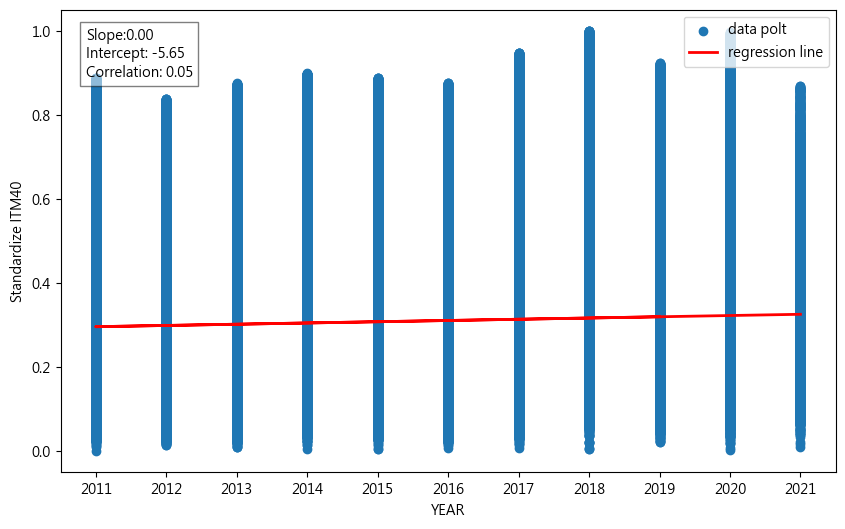
\includegraphics[width=6cm]{YEAR.png} 
		\caption{Year} 
		\label{Fig.YEAR} 
		\end{figure}
		
		\subsubsection{REL}
The chart illustrates the relationship between Family Member Titles and income. The linear regression line in the chart exhibits a good fit, indicating a certain correlation between the head of household and income. The positive slope of the regression line suggests that a closer relationship with the head of household corresponds to higher income.
The Relationship with the Head of Household (REL) is a significant variable factor in this context. It serves well in explaining the variations in income.
		\begin{figure}[H]
		\centering
		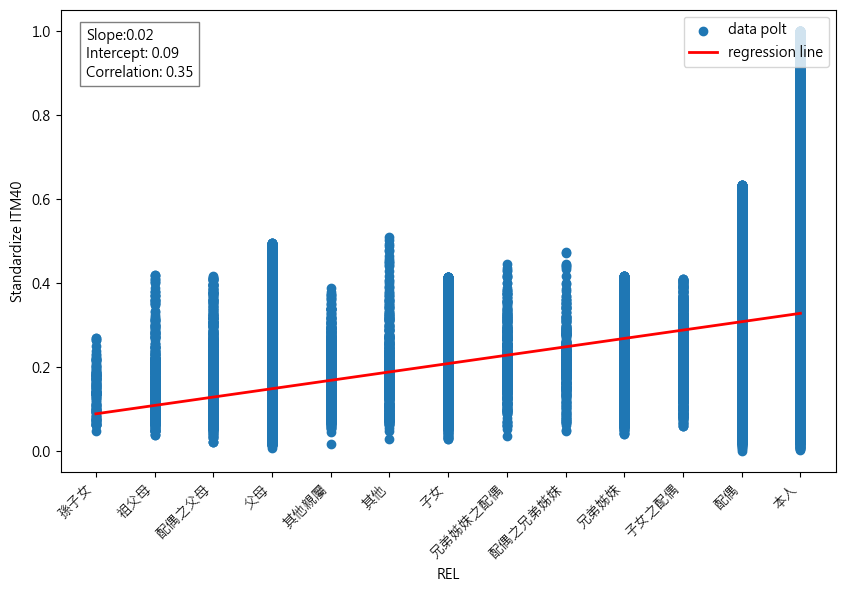
\includegraphics[width=6cm]{REL.png} 
		\caption{Family Member Titles} 
		\label{Fig.REL} 
		\end{figure}
		
		\subsubsection{SEX}
The chart illustrates the relationship between gender and income. The linear regression line in the chart shows a good fit, and the positive slope of the regression line indicates that men have higher incomes than women. In the low-income range, women's incomes are slightly higher than men's. However, in the high-income range, men's incomes are significantly higher than women's. Gender proves to be a significant variable factor, effectively explaining the differences in income.
		\begin{figure}[H]
		\centering
		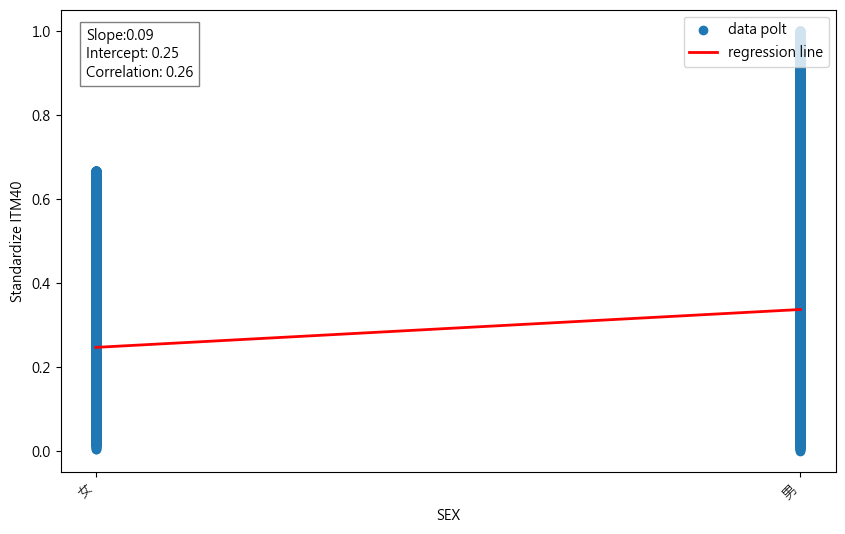
\includegraphics[width=6cm]{SEX.png} 
		\caption{Sex} 
		\label{Fig.SEX} 
		\end{figure}

		\subsubsection{AGE}
The chart depicts the relationship between age and income, and several observations can be made. It is evident from the chart that individuals between the ages of 50 and just before 60 have the highest income, forming a distribution resembling a normal curve. There is a steep ascending curve before the age of 50, and after the age of 60, the pattern resembles a quadratic curve. Therefore, we have employed a cubic function to better fit and express the distribution in the chart.
		\begin{figure}[H]
		\centering
		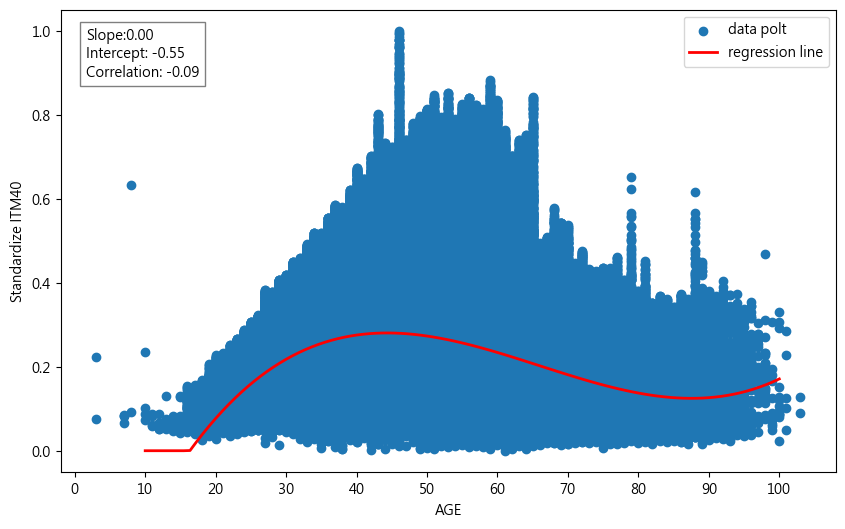
\includegraphics[width=6cm]{AGE.png} 
		\caption{Age} 
		\label{Fig.AGE} 
		\end{figure}
		
		\subsubsection{EDU}
This chart illustrates the relationship between education level and income. It is evident from the chart that a higher level of education corresponds to a higher income, aligning with common knowledge. Therefore, we believe that education level not only serves as a good differentiating variable but also conveys the importance of pursuing further education.		
		\begin{figure}[H]
		\centering
		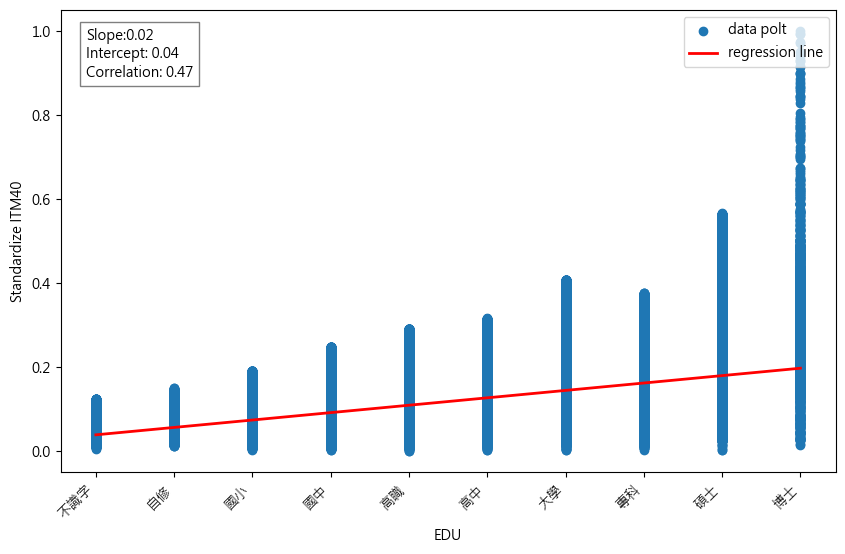
\includegraphics[width=6cm]{EDU.png} 
		\caption{Education} 
		\label{Fig.EDU} 
		\end{figure}
		
		\subsubsection{IND}
This chart depicts the relationship between industries and income. The chart is organized based on the average income for each industry. While there is a clear variation in income levels among different industries, some industries exhibit a broader distribution. For instance, the healthcare and social assistance industry shows a wide range between the upper and lower limits. The real estate industry, on the other hand, has a higher upper limit with a relatively smaller population.
These variations, especially in industries like healthcare and social assistance services, and real estate, may pose challenges to our predictions due to their wide income ranges and potentially lower sample sizes.
		\begin{figure}[H]
		\centering
		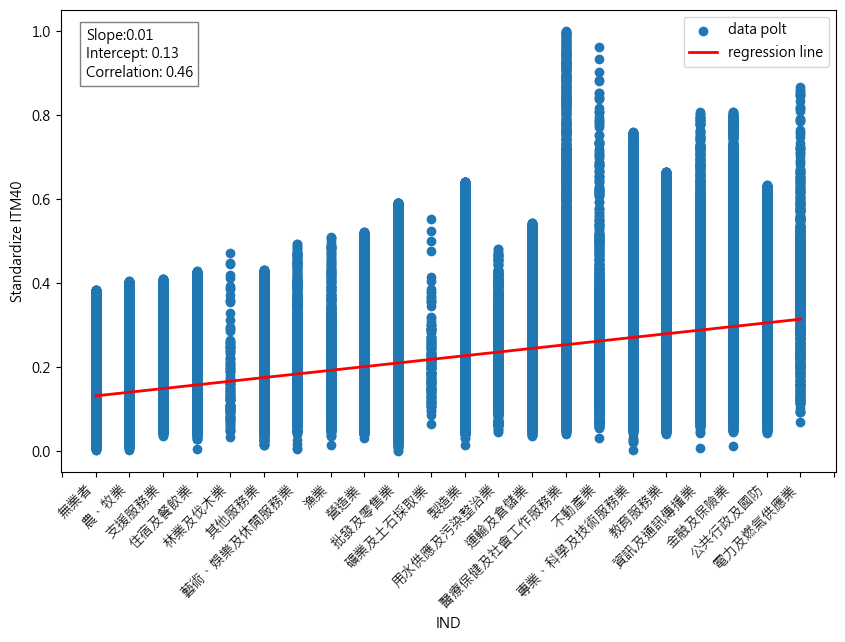
\includegraphics[width=6cm]{IND.png} 
		\caption{Industries} 
		\label{Fig.IND} 
		\end{figure}
		
		\subsubsection{OCC}
This chart illustrates the relationship between occupation and income. Similar to the industry chart, this one also ranks average incomes by occupation. Besides confirming that the incomes of representatives, supervisors, and managers are significantly higher than those in other occupations, the chart also informs us that frontline workers and production personnel tend to have lower salaries.
		\begin{figure}[H]
		\centering
		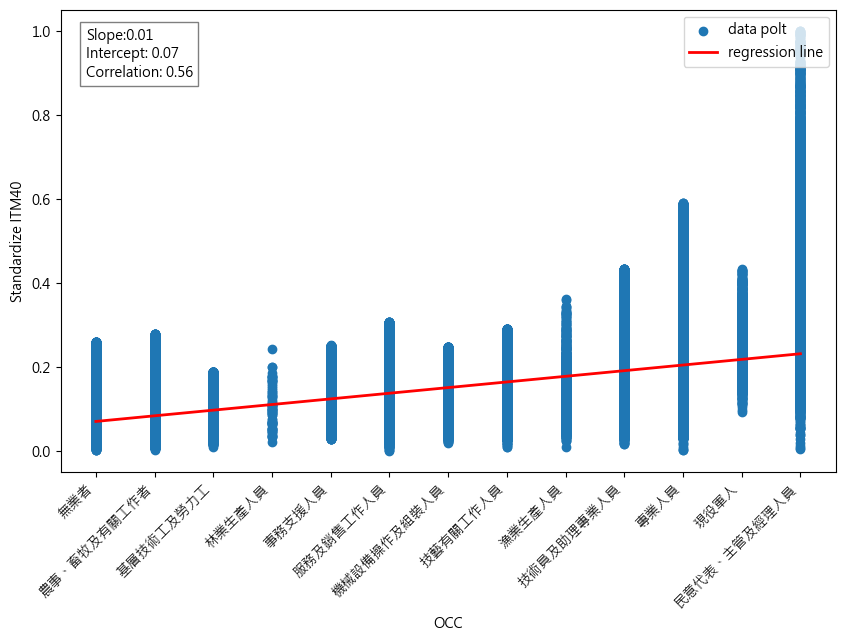
\includegraphics[width=6cm]{OCC.png} 
		\caption{Occupation} 
		\label{Fig.OCC} 
		\end{figure}
		
		\subsubsection{WKClass}
This chart depicts the relationship between different Employment Role and income. The categories, listed from least to greatest, include students, unpaid family workers, unemployed individuals, homemakers, self-employed individuals, employees, employers, and others. Notably, the income of employers is the highest among these categories, surpassing the others by a significant margin, even doubling the income of the second-highest category.
		\begin{figure}[H]
		\centering
		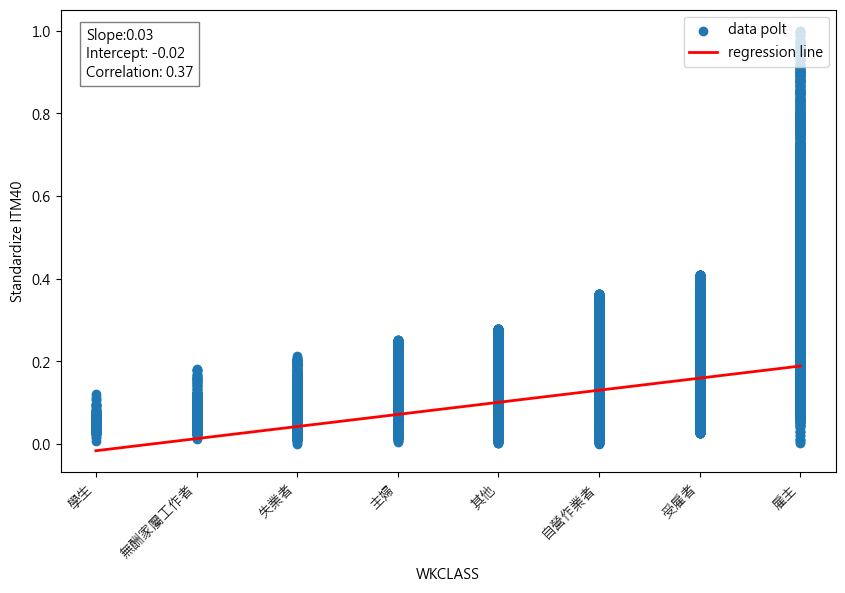
\includegraphics[width=6cm]{WKCLASS.png} 
		\caption{Employment Role} 
		\label{Fig.WKCLASS} 
		\end{figure}
		
		\subsubsection{WORK}
This chart illustrates the relationship between employment status and income. It shows that individuals who are employed tend to have higher incomes compared to those who are not employed.
		\begin{figure}[H]
		\centering
		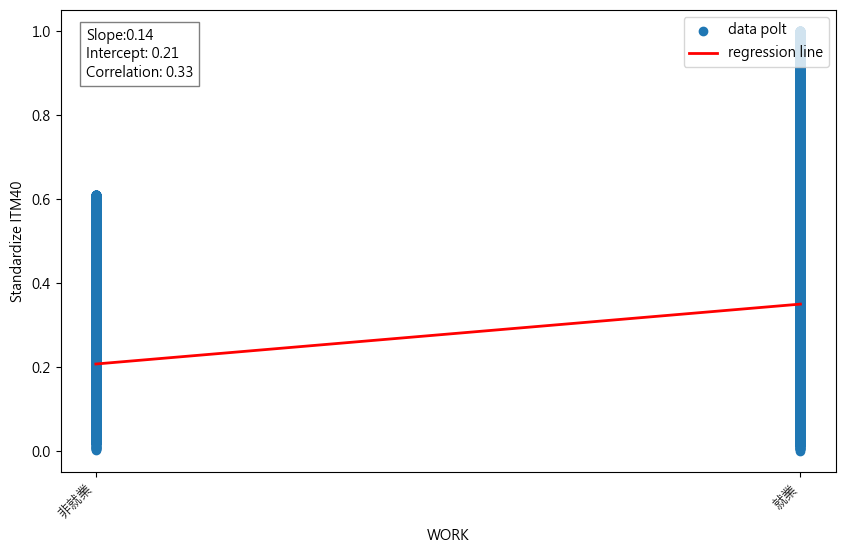
\includegraphics[width=6cm]{WORK.png} 
		\caption{Work or not} 
		\label{Fig.WORK} 
		\end{figure}

		\subsubsection{WORKPlace}
This chart depicts the relationship between the work location in Taiwan (local, foreign, northern region, central region, southern region) and income. It shows that working abroad is associated with the highest income, followed by the northern region and special municipalities, which generally have relatively higher incomes. Conversely, some more peripheral areas in the central and southern regions, as well as individuals who have received a one-time retirement pension, tend to have lower incomes.
		\begin{figure}[H]
		\centering
		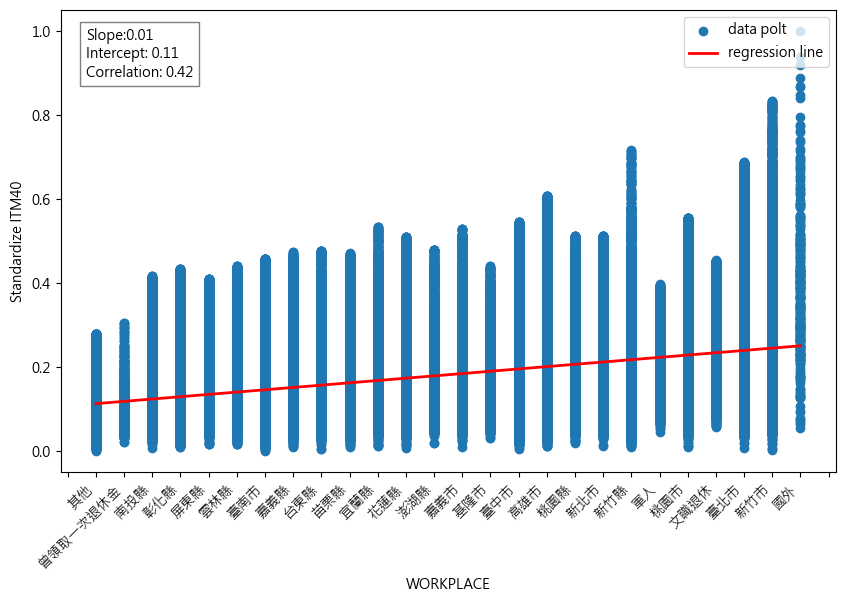
\includegraphics[width=6cm]{WORKPLACE.png} 
		\caption{Work Place} 
		\label{Fig.WORKPLACE} 
		\end{figure}

		\subsubsection{MRG}
This chart illustrates the relationship between marital status and income. It shows that the income for the married category is generally higher compared to the unmarried category. This suggests that marital status may indicate that both partners have income sources, making the overall income higher compared to unmarried individuals who rely on a single income source.
		\begin{figure}[H]
		\centering
		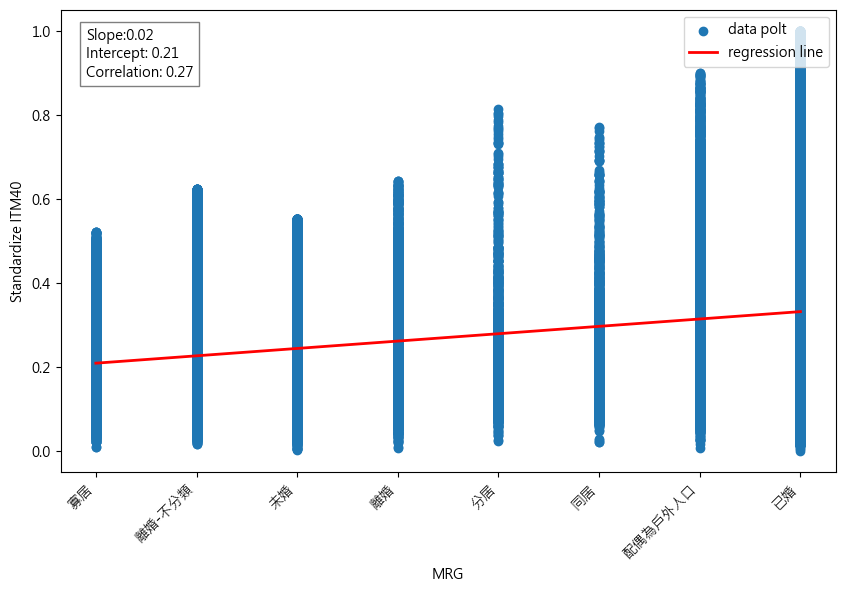
\includegraphics[width=6cm]{MRG.png} 
		\caption{marital status} 
		\label{Fig.MRG} 
		\end{figure}

		\subsubsection{PT}
This chart describes the relationship between having multiple jobs (moonlighting) and income. Clearly, individuals with multiple jobs have a higher income compared to those without additional employment.
		\begin{figure}[H]
		\centering
		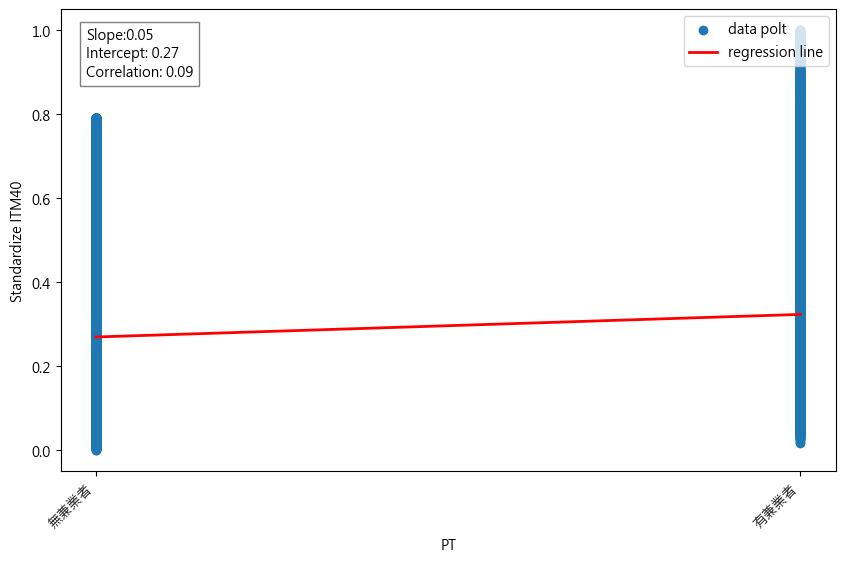
\includegraphics[width=6cm]{PT.png} 
		\caption{Have side job or not} 
		\label{Fig.PT} 
		\end{figure}
		
\section{Methodology}
	\subsection{tree Models}
The realm of machine learning is enriched by the diverse models encapsulated within the tree-based models. In this section, we delve into the intricacies of these models, exploring their principles, unique features, and applications in real-world scenarios. From the foundational Decision Tree Classifier and Regressor to the specialized Extremely Tree Classifier and Regressor, each model contributes to this paper. Through empirical evaluations and in-depth analyses, we aim to shed light on the strengths and nuances of these decision tree-based models, providing insights that contribute to the broader discourse on machine learning methodologies.
		\subsubsection{Decision Tree Regressor}
The Decision Tree Regressor, a fundamental member of the decision tree-based models in machine learning, operates on the principle of recursive binary splitting to approximate a continuous target variable. Let \(X\) represent the input features and \(Y\) the target variable, and consider a training dataset \(\{(X_i, Y_i)\}_{i=1}^{N}\). The goal is to construct a tree-based model, where each internal node represents a decision based on a selected feature, and each leaf node provides the predicted value.

The model's prediction is defined by traversing the decision tree from the root to a leaf node:

\[ \hat{Y}(x) = \text{Leaf}(x), \]

where \(x\) is an input instance, and \(\text{Leaf}(x)\) is the leaf node reached by the decision path.

The unique feature of the Decision Tree Regressor lies in its adaptability to capture complex nonlinear relationships in the data through a series of binary decisions. This adaptability is achieved by recursively splitting the feature space into regions, optimizing the splits based on the reduction in variance of the target variable.

Applications of Decision Tree Regressor are diverse, ranging from predicting housing prices and stock market trends to optimizing resource allocation in industrial processes. Its ability to handle numerical and categorical features, along with its interpretability, makes it a valuable tool in scenarios where understanding the underlying decision process is crucial.

In summary, the Decision Tree Regressor's distinctive strength lies in its hierarchical structure, enabling it to model intricate relationships in the data through recursive binary splits and providing interpretable insights into the decision-making process.

		\subsubsection{Extremely Tree Regressor}
The Extremely Tree Regressor, an extension of traditional decision tree models, distinguishes itself through an added layer of extreme randomness during the training process. Let \(X\) denote the input features, \(Y\) the continuous target variable, and consider a training dataset \(\{(X_i, Y_i)\}_{i=1}^{N}\). The objective is to build an ensemble of trees to approximate the target variable through additive predictions.

The prediction of the Extremely Tree Regressor is defined as:

\[ \hat{Y}(x) = \sum_{m=1}^{M} \gamma_m h_m(x), \]

where \(M\) is the number of trees, \(\gamma_m\) is the weight associated with each tree, and \(h_m(x)\) is the prediction of the \(m\)-th tree.

The uniqueness of the Extremely Tree Regressor lies in its introduction of extreme randomness during the tree-building process. Specifically, at each node, a random subset of features is considered for splitting, and the splitting threshold is chosen randomly. This heightened randomness enhances the diversity among individual trees and helps mitigate overfitting, contributing to a more robust ensemble.

Applications of the Extremely Tree Regressor span domains where predictive accuracy and resilience to noise are crucial. Its capacity to handle high-dimensional data, coupled with its efficient training process, makes it well-suited for tasks such as stock price prediction, energy consumption forecasting, and any regression problem requiring adaptability to complex relationships.

In summary, the Extremely Tree Regressor's distinctive strength lies in its extreme randomization, which enhances the diversity of individual trees, thereby providing a powerful tool for accurate and robust regression across various applications.

	\subsection{Svm Models}
Support Vector Machine (SVM) algorithms offer a powerful framework for both classification and regression tasks. This collection includes various SVM-based models, such as LinearSVR and SVR for linear regression, NuSVR for nu-support vector regression. These models operate on the principle of maximizing the margin between different classes or fitting a hyperplane to approximate a target variable. In this section, we delve into the principles, unique features, and diverse applications of SVM algorithms, exploring their effectiveness in solving real-world problems across different domains.
		\subsubsection{SVR}
Support Vector Regression (SVR) is a powerful regression algorithm belonging to the family of Support Vector Machines (SVM). Operating on the principles of structural risk minimization, SVR seeks to find a hyperplane that best fits the training data while allowing for a specified tolerance in errors. Let \(X\) denote the input features, \(Y\) the target variable, and \(\{(X_i, Y_i)\}_{i=1}^{N}\) the training dataset.

The objective of SVR is to find a function \(f(X)\) that minimizes the following optimization problem:

\[ \min_{f \in \mathcal{H}} \frac{1}{2} \|f\|^2 + C \sum_{i=1}^{N} \left(\xi_i + \xi_i^*\right), \]

subject to the constraints:

\[
\begin{aligned}
Y_i - f(X_i) &\leq \varepsilon + \xi_i, \\
f(X_i) - Y_i &\leq \varepsilon + \xi_i^*, \\
\xi_i, \xi_i^* &\geq 0,
\end{aligned}
\]

where \(\varepsilon\) is the specified tolerance, \(C\) is the regularization parameter, and \(\xi_i\) and \(\xi_i^*\) are slack variables.

The uniqueness of SVR lies in its ability to capture complex relationships in the data by identifying a hyperplane (or nonlinear decision boundary in the feature space) that minimizes the loss while allowing for deviations within the specified tolerance. This tolerance is controlled by the parameter \(\varepsilon\), enabling SVR to adapt to varying degrees of noise in the data.

Applications of SVR are diverse, ranging from financial forecasting to bioinformatics. Its adaptability to nonlinear relationships and robustness in handling outliers make it particularly well-suited for regression tasks where capturing intricate patterns and maintaining predictive accuracy are paramount.

In summary, Support Vector Regression's distinctive strength lies in its optimization framework, seeking a hyperplane that minimizes errors within a specified tolerance, and its versatility in capturing complex nonlinear relationships in diverse regression applications.

		\subsubsection{NuSVR}
Nu Support Vector Regression (NuSVR) is a variant of Support Vector Regression (SVR) that introduces a nu-parameter, providing a more flexible approach to controlling the number of support vectors and, consequently, the complexity of the regression model. Operating within the framework of Support Vector Machines (SVM), NuSVR seeks to find a hyperplane that approximates the target variable while allowing for deviations within a specified tolerance. Let \(X\) represent the input features, \(Y\) the target variable, and \(\{(X_i, Y_i)\}_{i=1}^{N}\) the training dataset.

The objective of NuSVR is to find a function \(f(X)\) that minimizes the following optimization problem:

\[ \min_{f \in \mathcal{H}} \frac{1}{2} \|f\|^2 + C \sum_{i=1}^{N} \left(\xi_i + \xi_i^*\right), \]

subject to the constraints:

\[
\begin{aligned}
Y_i - f(X_i) &\leq \varepsilon + \xi_i, \\
f(X_i) - Y_i &\leq \varepsilon + \xi_i^*, \\
\xi_i, \xi_i^* &\geq 0, \\
\frac{1}{N} \sum_{i=1}^{N} (\xi_i + \xi_i^*) &\leq \nu,
\end{aligned}
\]

where \(\varepsilon\) is the specified tolerance, \(C\) is the regularization parameter, \(\xi_i\) and \(\xi_i^*\) are slack variables, and \(\nu\) is the nu-parameter controlling the upper bound on the fraction of margin errors and support vectors.

The uniqueness of NuSVR lies in its nu-parameter, offering a more intuitive control over model complexity. By adjusting \(\nu\), practitioners can influence the trade-off between fitting the training data and allowing for deviations within the specified tolerance.

Applications of NuSVR extend across diverse domains, including finance and environmental modeling. Its adaptability to different levels of noise and its ability to control the number of support vectors make it valuable for regression tasks where striking the right balance between model complexity and generalization is crucial.

In summary, Nu Support Vector Regression's distinctive strength lies in its incorporation of the nu-parameter, providing a flexible mechanism to control the trade-off between model complexity and accuracy in regression applications.

		\subsubsection{Linear SVR}
Linear Support Vector Regression (Linear SVR) is a regression algorithm that leverages the principles of Support Vector Machines (SVM) to approximate a continuous target variable with a linear decision boundary. Operating within the framework of structural risk minimization, Linear SVR seeks to find a hyperplane that maximally preserves the margin between instances while minimizing deviations within a specified tolerance. Let \(X\) represent the input features, \(Y\) the target variable, and \(\{(X_i, Y_i)\}_{i=1}^{N}\) the training dataset.

The objective of Linear SVR is to find a linear function \(f(X)\) that minimizes the following optimization problem:

\[ \min_{f \in \mathcal{H}} \frac{1}{2} \|f\|^2 + C \sum_{i=1}^{N} \left(\max(0, |Y_i - f(X_i)| - \varepsilon)\right), \]

subject to the constraints:

\[ |Y_i - f(X_i)| \leq \varepsilon, \]

where \(\varepsilon\) is the specified tolerance, \(C\) is the regularization parameter, and \(\mathcal{H}\) is the space of linear functions.

The uniqueness of Linear SVR lies in its simplicity and interpretability, as it seeks a linear hyperplane in the feature space to model the relationship between input features and the target variable. This linearity makes Linear SVR particularly effective when the underlying relationship is approximately linear.

Applications of Linear SVR are widespread, including areas such as finance and economics. Its straightforward interpretation of the learned coefficients and efficiency in high-dimensional spaces make it valuable for regression tasks where transparency and computational efficiency are crucial.

In summary, Linear Support Vector Regression's distinctive strength lies in its linear decision boundary, providing a clear and interpretable solution for regression problems while maintaining the robustness and generalization capabilities of Support Vector Machines.

	\subsection{Neighbors Models}
The landscape of machine learning is enriched by the diversity of models, and among them, the k-nearest neighbors (KNN) algorithm stands out as a powerful and intuitive approach. The arsenal of KNN-based models, encapsulated such as BallTree and KDTree for efficient neighbor searches, KNeighborsRegressor for regression tasks, NearestCentroid for centroid-based classification, and LocalOutlierFactor for detecting outliers. In this section, we explore the principles, unique features, and applications of these KNN models, showcasing their versatility in solving regression, and anomaly detection challenges across diverse domains.
		\subsubsection{KNeighbors Regressor}
The KNeighbors Regressor is a powerful regression algorithm that operates on the simple yet effective principle of utilizing the information from the k-nearest neighbors to predict the continuous target variable. Given a dataset \(\{(X_i, Y_i)\}_{i=1}^{N}\), where \(X\) represents the input features and \(Y\) the target variable, the KNeighbors Regressor aims to estimate \(Y\) for a new instance \(x\) by averaging the target values of its k-nearest neighbors.

Mathematically, the prediction \(\hat{Y}(x)\) is defined as:

\[ \hat{Y}(x) = \frac{1}{k} \sum_{i=1}^{k} Y_{i'}, \]

where \(Y_{i'}\) represents the target value of the \(i'\)-th nearest neighbor to \(x\).

The unique feature of the KNeighbors Regressor lies in its adaptability to local data patterns, making it particularly effective in capturing non-linear relationships in the data. By adjusting the parameter \(k\), practitioners can control the level of local granularity, influencing the balance between model bias and variance.

Applications of KNeighbors Regressor are diverse, spanning fields such as real estate, finance, and environmental modeling. Its ability to adapt to local variations in data and provide interpretable predictions makes it well-suited for regression tasks where understanding localized patterns is crucial.

In summary, the KNeighbors Regressor's distinctive strength lies in its simplicity and adaptability, leveraging the information from nearby instances to provide accurate and locally-informed predictions in various regression scenarios.
		\subsubsection{Weighted Kneighbors Regressor}
Our approach aims to refine the K-Nearest Neighbors (KNN) algorithm by considering the varying influence of each feature on the target variable, ITM40. Instead of the conventional KNN method that treats all features equally, we enhance the model as follows:

We preprocess the data by applying one-hot encoding to categorical features and introducing a bias term. Linear regression is then employed to predict ITM40, Extremelycting feature weights in the process.

The obtained feature weights are incorporated into the KNN algorithm, allowing for a more nuanced distance calculation that considers the varying impact of each feature. This modification provides a refined measure of similarity between data points.

	\subsection{Linear Models}
In the realm of machine learning, a rich array of linear models forms the backbone of predictive modeling. This extensive collection includes a diverse set of algorithms, each tailored to address specific challenges in regression, classification, and more. From traditional linear regression models like LinearRegression and Ridge to advanced techniques such as BayesianRidge and ElasticNet, these models span a spectrum of methodologies. Whether dealing with logistic regression (LogisticRegression), robust regression (HuberRegressor), or sparse models (Lasso), this comprehensive suite offers a versatile toolkit to accommodate various data characteristics. In this section, we delve into the principles, unique characteristics, and practical applications of these linear models, aiming to unravel the intricacies of their diverse functionalities and contributions to the landscape of machine learning.
		\subsubsection{Linear Regression}
Linear Regression, a fundamental and widely-used model in the realm of machine learning, operates on the principle of modeling the relationship between the input features \(X\) and the continuous target variable \(Y\) through a linear function. Given a dataset \(\{(X_i, Y_i)\}_{i=1}^{N}\), where \(N\) is the number of instances, Linear Regression aims to find the coefficients \(\beta_0, \beta_1, \ldots, \beta_p\) that minimize the sum of squared differences between the predicted and actual target values.

Mathematically, the linear regression model is represented as:

\[ \hat{Y}(X) = \beta_0 + \beta_1 X_1 + \beta_2 X_2 + \ldots + \beta_p X_p, \]

where \(\hat{Y}(X)\) is the predicted target value, \(X_1, X_2, \ldots, X_p\) are the input features, and \(\beta_0, \beta_1, \ldots, \beta_p\) are the coefficients.

The unique feature of Linear Regression lies in its simplicity and interpretability. The coefficients \(\beta_i\) indicate the contribution of each feature to the predicted output, offering insights into the strength and direction of the relationships. Moreover, Linear Regression assumes a linear relationship between the features and the target, making it suitable for scenarios where such linearity holds.

Applications of Linear Regression are ubiquitous, ranging from predicting housing prices based on features like square footage and location to estimating sales figures based on advertising budgets. Its straightforward interpretation, computational efficiency, and ability to capture linear relationships make it a cornerstone in various regression tasks where a clear understanding of feature contributions is essential.

In summary, Linear Regression's distinctive strength lies in its straightforward representation of linear relationships, providing a transparent and interpretable framework for predicting continuous target variables in diverse real-world applications.

		\subsubsection{RANSAC Regressor}
The RANSAC (Random Sample Consensus) Regressor is a robust regression algorithm designed to mitigate the impact of outliers on model performance. In the presence of noisy data or outliers, traditional regression models may yield inaccurate results. RANSAC addresses this challenge by iteratively fitting models to random subsets of the data, known as inliers, while identifying and discarding outliers.

Given a dataset \(\{(X_i, Y_i)\}_{i=1}^{N}\) where \(X\) represents the input features and \(Y\) is the continuous target variable, RANSAC seeks to find the coefficients \(\beta_0, \beta_1, \ldots, \beta_p\) that minimize the sum of squared differences only for the inliers.

Mathematically, the RANSAC regression model is represented as:

\[ \hat{Y}(X) = \beta_0 + \beta_1 X_1 + \beta_2 X_2 + \ldots + \beta_p X_p, \]

where \(\hat{Y}(X)\) is the predicted target value, and \(X_1, X_2, \ldots, X_p\) are the input features.

The RANSAC algorithm works iteratively by randomly sampling a subset of the data, fitting a model, identifying inliers based on a predefined threshold, and repeating this process to find the best-fitting model. This iterative approach makes RANSAC robust to outliers and noise in the dataset.

The unique feature of RANSAC lies in its ability to provide reliable regression estimates even in the presence of a significant number of outliers. This makes it particularly valuable in applications where the dataset may contain noise or anomalies, such as computer vision tasks or sensor data processing.

Applications of RANSAC Regressor extend to various fields, including image processing, robotics, and computer graphics. Its resilience to outliers and its capability to yield accurate regression results in the presence of noisy data make it a go-to choice for scenarios where data quality may be compromised.

In summary, RANSAC Regressor's distinctive strength lies in its robustness to outliers, achieved through an iterative process that selectively fits models to inliers, making it an invaluable tool for regression tasks in the presence of noisy or contaminated datasets.

		\subsubsection{Huber Regressor}
The Huber Regressor is a robust regression algorithm designed to strike a balance between the mean squared error (MSE) and the mean absolute error (MAE), providing resilience to outliers while maintaining the efficiency of traditional least squares regression. Operating on a dataset \(\{(X_i, Y_i)\}_{i=1}^{N}\) with input features \(X\) and a continuous target variable \(Y\), the Huber Regressor seeks to find the coefficients \(\beta_0, \beta_1, \ldots, \beta_p\) that minimize the Huber loss function.

Mathematically, the Huber loss function is defined as:

\[ L_{\delta}(y, f(X)) = \begin{cases} 
\frac{1}{2}(y - f(X))^2 & \text{for } |y - f(X)| \leq \delta, \\
\delta \cdot |y - f(X)| - \frac{1}{2}\delta^2 & \text{otherwise,}
\end{cases} \]

where \(f(X)\) is the predicted target value, \(y\) is the true target value, and \(\delta\) is a threshold parameter that determines the point of transition between the quadratic and linear loss regions.

The Huber Regressor adapts to the characteristics of the data by penalizing large errors with a quadratic loss for inliers and a linear loss for outliers. This unique feature makes it robust to the influence of extreme values while still providing a smooth transition between regions.

Applications of Huber Regressor are prevalent in fields where data may contain outliers, such as finance and environmental modeling. Its adaptability to different levels of noise and outliers, combined with the computational efficiency of least squares regression, positions it as a versatile tool for robust regression tasks.

In summary, Huber Regressor's distinctive strength lies in its ability to balance the trade-off between mean squared error and mean absolute error, making it a robust choice for regression tasks in the presence of outliers and noisy data.

		\subsubsection{Poisson Regressor}
The Poisson Regressor is a specialized regression model designed for count data, where the response variable represents the number of occurrences of a specific event in a fixed interval. Operating within the framework of a dataset \(\{(X_i, Y_i)\}_{i=1}^{N}\) with input features \(X\) and a count target variable \(Y\), the Poisson Regressor is tailored to model the distribution of count data.

The Poisson regression model assumes that the count variable \(Y\) follows a Poisson distribution with a mean parameter \(\lambda\). The relationship between the input features \(X\) and the mean parameter \(\lambda\) is modeled using the exponential function:

\[ \lambda = e^{\beta_0 + \beta_1 X_1 + \beta_2 X_2 + \ldots + \beta_p X_p}, \]

where \(\beta_0, \beta_1, \ldots, \beta_p\) are the coefficients to be estimated.

The unique feature of the Poisson Regressor lies in its suitability for count data, addressing the specific characteristics of non-negative integers. Unlike traditional linear regression models, the Poisson Regressor accommodates the discrete nature of count outcomes and ensures that predicted values align with the inherent properties of count data.

Applications of the Poisson Regressor are prevalent in fields such as epidemiology, finance, and traffic modeling, where the goal is to predict the number of events or occurrences within a given timeframe. Its adaptability to count data and its provision of interpretable results make it a valuable tool for regression tasks where count outcomes are of primary interest.

In summary, the Poisson Regressor's distinctive strength lies in its specialized modeling of count data, leveraging the Poisson distribution to provide accurate predictions for scenarios where the response variable represents the frequency of specific events.

		\subsubsection{Passive Aggressive Regressor}
The Passive Aggressive Regressor is a dynamic and adaptive regression algorithm designed for online learning scenarios where data arrives sequentially. Operating on a dataset \(\{(X_i, Y_i)\}_{i=1}^{N}\) with input features \(X\) and continuous target variable \(Y\), the Passive Aggressive Regressor updates its model iteratively, accommodating new observations while remaining computationally efficient.

The update rule for the Passive Aggressive Regressor is defined as follows:

\[ w_{t+1} = w_t + \eta \cdot \max(0, 1 - \frac{Y_t \cdot \langle w_t, X_t \rangle}{||X_t||_2^2}) \cdot Y_t \cdot X_t, \]

where \(w_t\) is the weight vector at time \(t\), \(\eta\) is the learning rate, \(Y_t\) is the true target value, and \(X_t\) represents the input features of the current observation.

The unique feature of the Passive Aggressive Regressor lies in its ability to handle new data points adaptively. It introduces a margin parameter, allowing the model to adjust its weights based on the loss incurred for a given observation. This adaptability is particularly beneficial in situations where the data distribution may change over time.

Applications of the Passive Aggressive Regressor are prominent in online learning scenarios, such as dynamic financial modeling and streaming data analysis. Its capacity to swiftly adapt to changing patterns in data and its efficiency in processing sequentially arriving observations make it well-suited for real-time regression tasks.

In summary, the Passive Aggressive Regressor's distinctive strength lies in its adaptability to dynamic environments, offering a computationally efficient solution for online learning scenarios where model updates are required in response to sequentially arriving data.

		\subsubsection{TheilSen Regressor}
The TheilSen Regressor is a robust linear regression algorithm that excels in the presence of outliers. Operating on a dataset \(\{(X_i, Y_i)\}_{i=1}^{N}\) with input features \(X\) and a continuous target variable \(Y\), the TheilSen Regressor seeks to estimate the slope and intercept of the underlying linear relationship by calculating the median of the slopes obtained from all pairs of data points.

Mathematically, the slope (\(b\)) and intercept (\(a\)) of the TheilSen regression line are determined as follows:

\[ b = \text{median}\left(\frac{Y_j - Y_i}{X_j - X_i}\right), \]
\[ a = \text{median}(Y_i - b \cdot X_i), \]

where \(i\) and \(j\) represent distinct pairs of data points.

The unique feature of the TheilSen Regressor lies in its robustness to outliers. By using the median instead of the mean to calculate both the slope and intercept, the algorithm minimizes the impact of extreme values, providing a more accurate estimate of the underlying linear trend. This robustness makes it well-suited for scenarios where the data may contain influential outliers.

Applications of the TheilSen Regressor are prevalent in fields such as environmental modeling and finance, where the presence of outliers can significantly affect the accuracy of linear regression models. Its resilience to extreme values and its ability to provide reliable linear estimates make it a valuable tool for robust regression tasks.

In summary, the TheilSen Regressor's distinctive strength lies in its robustness to outliers, achieved through the use of median-based estimators for both slope and intercept, making it a reliable choice for linear regression in the presence of influential data points.

		\subsubsection{Bayesian Ridge}
The Bayesian Ridge Regressor is a Bayesian approach to linear regression that incorporates regularization, providing a principled framework for handling multicollinearity and preventing overfitting. Operating on a dataset \(\{(X_i, y_i)\}_{i=1}^{N}\) with input features \(X\) and continuous target variable \(y\), the Bayesian Ridge Regressor estimates the linear relationship between the features and the target by modeling the weights as random variables with a Gaussian prior.

The Bayesian Ridge regression model is defined as follows:

\[ y = X \beta + \epsilon, \]
\[ \beta \sim \mathcal{N}(0, \alpha^{-1}I), \]
\[ \epsilon \sim \mathcal{N}(0, \lambda^{-1}I), \]

where \(y\) is the target variable, \(X\) is the design matrix, \(\beta\) represents the regression coefficients, and \(\epsilon\) is the error term. The hyperparameters \(\alpha\) and \(\lambda\) control the precision of the prior distributions.

The unique feature of Bayesian Ridge lies in its Bayesian formulation, which allows for the incorporation of prior knowledge about the distribution of weights. The regularization term introduced by the prior mitigates multicollinearity and provides a natural way to control model complexity.

Applications of Bayesian Ridge are widespread in situations where interpretability of the model and handling multicollinearity are essential, such as finance and epidemiology. Its probabilistic framework facilitates uncertainty estimation in predictions, making it suitable for scenarios where a measure of prediction confidence is valuable.

In summary, the Bayesian Ridge Regressor's distinctive strength lies in its Bayesian approach to linear regression, providing a robust and interpretable solution that effectively handles multicollinearity and prevents overfitting through the incorporation of prior knowledge about the distribution of weights.

		\subsubsection{Elastic Net}
The Elastic Net Regressor is a regularization technique that combines both L1 (Lasso) and L2 (Ridge) regularization penalties, providing a flexible and robust approach to linear regression. Operating on a dataset \(\{(X_i, y_i)\}_{i=1}^{N}\) with input features \(X\) and continuous target variable \(y\), the Elastic Net Regressor addresses multicollinearity and feature selection challenges by introducing a combination of both L1 and L2 regularization terms.

The objective function of the Elastic Net regression model is defined as follows:

\[ \min_{\beta} \left\{ \frac{1}{2N} \|y - X\beta\|_2^2 + \alpha \rho \| \beta \|_1 + \frac{\alpha(1-\rho)}{2} \| \beta \|_2^2 \right\}, \]

where \(y\) is the target variable, \(X\) is the design matrix, \(\beta\) represents the regression coefficients, \(\alpha\) controls the overall strength of regularization, and \(\rho\) determines the trade-off between L1 and L2 penalties.

The unique feature of Elastic Net lies in its ability to handle both variable selection and parameter shrinkage simultaneously. By combining the sparsity-inducing property of L1 regularization with the stabilizing effect of L2 regularization, Elastic Net provides a balanced solution that is particularly effective in scenarios where many features are correlated.

Applications of Elastic Net are widespread, especially in high-dimensional datasets where feature selection and regularization are critical. Fields such as genomics, finance, and image processing benefit from its ability to handle collinearity and select relevant features, leading to more interpretable and robust regression models.

In summary, the Elastic Net Regressor's distinctive strength lies in its dual regularization approach, offering a versatile solution for linear regression tasks that require both feature selection and regularization to handle multicollinearity.

	\subsection{Neural Network Models}
The landscape of machine learning has witnessed significant advancements with the rise of models based on neural networks. Among these, the "MLPRegressor" stand out as powerful contributors to the realm of artificial intelligence. The Multilayer Perceptron Regressor (MLPRegressor) models showcase the prowess of deep learning in handling complex classification and regression tasks. This section delves into the unique characteristics, training methodologies, and practical applications of these neural network-based models, shedding light on their roles in pushing the boundaries of machine learning capabilities.
		\subsubsection{MLP Regressor}
The Multilayer Perceptron Regressor (MLP Regressor) is a versatile neural network-based model designed for solving complex regression tasks. Operating on a dataset \(\{(X_i, y_i)\}_{i=1}^{N}\) with input features \(X\) and continuous target variable \(y\), the MLP Regressor leverages a multilayer feedforward architecture to learn intricate non-linear relationships between input features and the target.

The forward pass of the MLP Regressor can be expressed mathematically as follows:

\[ h_i = \sigma(W_i \cdot h_{i-1} + b_i), \]
\[ \hat{y} = W_{\text{out}} \cdot h_L + b_{\text{out}}, \]

where \(h_i\) represents the hidden layer activations, \(\sigma\) is the activation function, \(W_i\) and \(b_i\) are the weight matrix and bias vector for layer \(i\), and \(L\) denotes the number of hidden layers.

The unique feature of the MLP Regressor lies in its ability to capture complex relationships within the data through the presence of multiple hidden layers. Each hidden layer introduces non-linear transformations, enabling the model to learn and represent intricate patterns in the input space.

Applications of the MLP Regressor span a wide range of domains, including finance, healthcare, and engineering, where complex dependencies between variables necessitate a model capable of capturing non-linear trends. Its adaptability to various data structures and robustness in handling intricate regression tasks make it a valuable tool for predictive modeling in diverse real-world scenarios.

In summary, the MLP Regressor's distinctive strength lies in its multilayer feedforward architecture, allowing it to effectively model non-linear relationships in regression tasks and providing a powerful solution for capturing intricate patterns within complex datasets.
		
	\subsection{Cross Decomposition Models}
Partial Least Squares (PLS) methods represent a powerful suite of models within the realm of multivariate analysis. Specifically, "PLSRegression" stand out as key contributors to understanding and modeling relationships between two sets of variables. This section explores the principles and applications of these models, delving into their unique characteristics and showcasing their effectiveness in uncovering latent patterns and correlations within complex datasets. Through a comprehensive examination of these techniques, we aim to provide insights into their diverse applications and their roles in advancing multivariate analysis methodologies.
		\subsubsection{PLS Regression}
Partial Least Squares Regression (PLS Regression) is a powerful multivariate technique designed for modeling the relationships between two sets of variables. Operating on a dataset \(\{(X_i, Y_i)\}_{i=1}^{N}\) with input features \(X\) and target variables \(Y\), PLS Regression aims to find latent factors that capture the maximum covariance between the two sets.

The PLS Regression model is established through the following mathematical formulation:

\[ X = TP^T + E_X, \]
\[ Y = UQ^T + E_Y, \]
\[ \hat{Y} = Xb = TP^Tb, \]

where \(X\) and \(Y\) are the input and target matrices, respectively, \(T\) and \(U\) are the score matrices, \(P\) and \(Q\) are the loading matrices, \(b\) is the regression vector, and \(E_X\) and \(E_Y\) are the residual matrices.

The unique feature of PLS Regression lies in its iterative process of finding latent factors that simultaneously maximize the covariance between \(X\) and \(Y\). This enables the model to handle high-dimensional data and collinearity efficiently, making it suitable for scenarios where traditional regression models may struggle.

Applications of PLS Regression are widespread, ranging from chemometrics and bioinformatics to finance and marketing. Its ability to capture latent structures and handle multicollinearity makes it a valuable tool for predictive modeling when dealing with complex datasets and multiple correlated response variables.

In summary, PLS Regression's distinctive strength lies in its iterative approach to finding latent factors that maximize covariance, providing an efficient solution for modeling relationships between two sets of variables in high-dimensional and collinear data settings.

	\subsection{Ensemble Models}
This section introduces a comprehensive suite of ensemble-based methods for classification, regression. Ranging from traditional bagging techniques like Baggingv Regressor to sophisticated tree-based ensembles such as Random Forest Regressor. Additionally, boosting methods like Gradient Boosting Regressor, along with meta-ensemble strategies, contribute to the rich ensemble ecosystem. This section aims to explore the distinctive features and applications of these models.
		\subsubsection{Bagging Regressor}	
The Bagging Regressor, an ensemble learning technique, operates on the fundamental principle of Bootstrap Aggregating (Bagging). It stands out for its unique approach to reducing variance and enhancing model stability through the aggregation of multiple base regressors. 

Mathematically, let \(X\) denote the input features, \(Y\) the target variable, and \(\{ (X_i, Y_i) \}_{i=1}^{N}\) the training dataset. Bagging involves constructing \(B\) base regressors \(\{h_b(X)\}_{b=1}^{B}\), each trained on a bootstrapped subset of the training data. The final prediction is then obtained by averaging the predictions of all base regressors:

\[ \hat{Y}(x) = \frac{1}{B} \sum_{b=1}^{B} h_b(x), \]

where \(x\) is a new input instance. This ensemble averaging effectively reduces overfitting and improves the model's generalization performance.

The unique feature of Bagging Regressor lies in its emphasis on diversity among the base regressors. By training each base regressor on a different subset of the data, Bagging promotes decorrelation among the individual models, leading to an ensemble that is less sensitive to noise and outliers in the training set.

Applications of Bagging Regressor span various domains, including finance, healthcare, and environmental sciences. It excels in scenarios where predictive accuracy and robustness are crucial, making it well-suited for tasks such as stock price prediction, medical diagnosis, and environmental impact assessment.

In summary, the Bagging Regressor's distinctive strength lies in its application of Bootstrap Aggregating to build an ensemble of diverse base regressors, effectively reducing variance and enhancing overall predictive performance.
	
		\subsubsection{Random Forest Regressor}
The Random Forest Regressor, an extension of the random forest algorithm, is distinguished by its unique approach to ensemble learning and its capacity to address overfitting while maintaining predictive accuracy. Operating on the principle of building a multitude of decision trees, this regressor introduces randomness at multiple levels to enhance the robustness and generalization of the model.

Let \(X\) represent the input features, \(Y\) the target variable, and \(\{ (X_i, Y_i) \}_{i=1}^{N}\) the training dataset. Random Forest Regressor constructs \(B\) decision trees \(\{h_b(X)\}_{b=1}^{B}\) through bootstrapped subsets of the training data and random feature selection at each node. The final prediction is obtained by averaging the predictions of all individual trees:

\[ \hat{Y}(x) = \frac{1}{B} \sum_{b=1}^{B} h_b(x), \]

where \(x\) is a new input instance. The ensemble averaging mitigates the risk of overfitting by incorporating diverse decision trees.

The key feature of Random Forest Regressor lies in its decorrelated and diverse ensemble. The randomness introduced in both the data and feature space during training ensures that each tree captures different aspects of the underlying patterns in the data. This feature enhances the model's resistance to noise and outliers.

Random Forest Regressor finds applications across various domains, including finance, ecology, and bioinformatics. It excels in tasks where capturing complex relationships and handling high-dimensional data are essential, making it well-suited for applications such as stock price prediction, ecosystem modeling, and gene expression analysis.

In summary, the Random Forest Regressor's strength lies in its ensemble of decorrelated decision trees, introducing randomness at multiple levels to address overfitting, enhance robustness, and provide reliable predictions across diverse regression scenarios.
		
		\subsubsection{Extremely Trees Regressor}
The Extremely Trees Regressor, an extension of the random forest algorithm, distinguishes itself through its core principle of extreme randomization during the tree construction process. In contrast to traditional methods, this regressor introduces an unprecedented level of randomness both in feature selection at each node and in the determination of thresholds for those features. Mathematically, if \(X\) represents the input features and \(Y\) the target variable, the split point \(s\) is chosen at each node by:

\[ s = \text{random\_threshold}(X_i), \]

where \(X_i\) is a randomly selected feature. This heightened randomness contributes to the creation of trees that are not only diverse but also decorrelated, enhancing the ensemble's overall predictive power.

The regressor's uniqueness lies in its commitment to extreme randomness, fostering independence among trees and amplifying sensitivity to diverse feature patterns. The prediction for a given input \(x\) is then obtained by aggregating the predictions of all individual trees:

\[ \hat{Y}(x) = \frac{1}{N} \sum_{i=1}^{N} f_i(x), \]

where \(N\) is the number of trees and \(f_i(x)\) is the prediction of the \(i\)-th tree. This ensemble approach mitigates overfitting and enhances generalization, making it particularly effective in regression tasks.

Furthermore, the Extremely Trees Regressor offers robustness to outliers due to its inherent randomness, making it well-suited for applications such as anomaly detection. The integration of extreme randomness in both feature selection and threshold determination positions this regressor as a powerful and flexible tool, demonstrating its efficacy in capturing complex patterns and enhancing predictive performance in diverse regression scenarios.

		\subsubsection{Hist Gradient Boosting Regressor}
The Hist Gradient Boosting Regressor stands out as an advanced gradient boosting algorithm, designed to optimize efficiency and scalability while maintaining high predictive accuracy. Operating on the principle of iteratively boosting weak learners, this regressor introduces a histogram-based approach for enhanced computational performance.

Let \(X\) denote the input features, \(Y\) the target variable, and \(\{ (X_i, Y_i) \}_{i=1}^{N}\) the training dataset. The regressor aims to approximate the target variable through an additive model:

\[ \hat{Y}(x) = \sum_{m=1}^{M} \gamma_m h_m(x), \]

where \(M\) is the number of weak learners, \(\gamma_m\) is the associated weight, and \(h_m(x)\) is the weak learner. In Hist Gradient Boosting, each weak learner is a histogram of the data, and the model minimizes the L2 loss:

\[ L(\{ (X_i, Y_i) \}_{i=1}^{N}, \hat{Y}(x)) = \sum_{i=1}^{N} (Y_i - \hat{Y}(X_i))^2. \]

The unique feature of Hist Gradient Boosting lies in its use of histogram-based techniques to discretize and represent the data efficiently during the training process. This approach significantly accelerates computation by reducing the number of data points considered at each split, making it particularly effective for large datasets.

Applications of Hist Gradient Boosting Regressor span diverse domains, including finance, healthcare, and online advertising. Its efficiency and scalability make it well-suited for tasks such as predicting financial market trends, optimizing medical treatment plans, and enhancing personalized advertising strategies.

In summary, the Hist Gradient Boosting Regressor's distinctive strength lies in its use of histogram-based techniques for efficient computation during the boosting process, making it a powerful and scalable tool for accurate regression across various application domains.

		\subsubsection{Gradient Boosting Regressor}
The Gradient Boosting Regressor is a powerful machine learning algorithm known for its ability to sequentially build a strong predictive model by combining weak learners. Operating on the principle of minimizing the residual errors from the previous models, this regressor optimizes predictive accuracy through a weighted sum of weak learners.

Let \(X\) represent the input features, \(Y\) the target variable, and \(\{ (X_i, Y_i) \}_{i=1}^{N}\) the training dataset. The objective is to approximate the target variable through an additive model:

\[ \hat{Y}(x) = \sum_{m=1}^{M} \gamma_m h_m(x), \]

where \(M\) is the number of weak learners, \(\gamma_m\) is the associated weight, and \(h_m(x)\) is the weak learner. The model minimizes a loss function, often the mean squared error for regression tasks:

\[ L(\{ (X_i, Y_i) \}_{i=1}^{N}, \hat{Y}(x)) = \sum_{i=1}^{N} (Y_i - \hat{Y}(X_i))^2. \]

The unique feature of Gradient Boosting lies in its sequential training process, where each new weak learner is fit to the residual errors of the ensemble formed by the previous learners. This approach addresses the shortcomings of individual weak models, gradually improving the overall model's accuracy.

Applications of Gradient Boosting Regressor are widespread, spanning areas such as finance, healthcare, and marketing. It excels in tasks requiring high predictive accuracy, such as stock price prediction, patient outcome modeling, and customer churn prediction.

In summary, the Gradient Boosting Regressor's distinctive strength lies in its sequential training approach, leveraging the ensemble of weak learners to iteratively minimize residual errors and achieve superior predictive performance across diverse regression applications.

		\subsubsection{AdaBoost Regressor}
The AdaBoost Regressor is a boosting algorithm renowned for its ability to sequentially combine weak learners to create a robust and accurate predictive model. Operating on the principle of assigning weights to data points based on their performance, this regressor iteratively emphasizes the importance of mispredicted instances, enabling the construction of a strong ensemble model.

Let \(X\) represent the input features, \(Y\) the target variable, and \(\{ (X_i, Y_i) \}_{i=1}^{N}\) the training dataset. The AdaBoost Regressor constructs an additive model as follows:

\[ \hat{Y}(x) = \sum_{m=1}^{M} \alpha_m h_m(x), \]

where \(M\) is the number of weak learners, \(\alpha_m\) is the associated weight, and \(h_m(x)\) is the weak learner. The model minimizes an exponential loss function:

\[ L(\{ (X_i, Y_i) \}_{i=1}^{N}, \hat{Y}(x)) = \sum_{i=1}^{N} e^{-Y_i \cdot \hat{Y}(X_i)}. \]

The unique feature of AdaBoost lies in its adaptive weighting of data points, with mispredicted instances being assigned higher weights in subsequent iterations. This adaptability ensures that the algorithm focuses on improving the prediction accuracy for challenging examples.

Applications of AdaBoost Regressor span diverse domains, including finance, biology, and image processing. It excels in tasks where addressing the impact of outliers and improving overall model accuracy are critical, such as predicting financial market trends, modeling biological processes, and enhancing image regression tasks.

In summary, the AdaBoost Regressor's distinctive strength lies in its adaptive boosting process, which dynamically adjusts weights based on misclassification errors, leading to the creation of a robust and accurate ensemble model for regression tasks.

	\subsection{Popular Models(on Kaggle)}
In the realm of competitive machine learning on platforms like Kaggle, certain models have emerged as go-to choices for achieving high-performance results. Notably, "xgboost," "lightgbm," and "catboost" stand out as popular and effective gradient boosting frameworks. This paper explores the principles and applications of these models, delving into their unique features that have contributed to their prevalence in Kaggle competitions. As we navigate through the intricacies of boosting algorithms, we aim to uncover the distinct strengths and characteristics that make "xgboost," "lightgbm," and "catboost" preferred tools among data scientists and machine learning enthusiasts in the Kaggle community.
		\subsubsection{xgboost}
XGBoost, short for eXtreme Gradient Boosting, is a powerful and widely adopted gradient boosting framework designed for both regression and classification tasks. Operating on a dataset \(\{(X_i, y_i)\}_{i=1}^{N}\) with input features \(X\) and target variable \(y\), xgboost employs an ensemble of decision trees to make accurate and efficient predictions.

The objective function of xgboost is defined as a sum of a differentiable loss function \(L(y_i, \hat{y}_i)\) and a regularization term that penalizes the complexity of the model:

\[ \mathcal{L}(\theta) = \sum_{i=1}^{N} L(y_i, \hat{y}_i) + \sum_{k=1}^{K} \Omega(f_k), \]

where \(\theta\) represents the set of parameters in the ensemble, \(f_k\) denotes individual decision trees, and \(\Omega(f_k)\) is the regularization term.

The unique features of xgboost include its ability to handle missing values, regularization techniques to control overfitting, and a clever computation strategy that optimizes the tree construction process. Additionally, xgboost incorporates a mechanism for parallel and distributed computing, enhancing scalability and speed.

Applications of xgboost span a wide range of domains, from finance and healthcare to online advertising. Its success in Kaggle competitions attests to its effectiveness in handling diverse datasets and producing state-of-the-art predictive performance.

In summary, xgboost's distinctive strengths lie in its regularization techniques, handling of missing data, and efficient computation strategy, making it a popular and effective choice for boosting algorithms in both competitive machine learning and real-world applications.

		\subsubsection{lightgbm}
LightGBM, a powerful gradient boosting framework, has gained prominence for its efficiency and scalability, making it well-suited for large-scale machine learning tasks. Operating on a dataset \(\{(X_i, y_i)\}_{i=1}^{N}\) with input features \(X\) and target variable \(y\), LightGBM employs a novel tree construction algorithm and efficient data representation to achieve remarkable speed and accuracy.

The objective function of LightGBM is defined as a sum of a differentiable loss function \(L(y_i, \hat{y}_i)\) and a regularization term that controls the complexity of the model:

\[ \mathcal{L}(\theta) = \sum_{i=1}^{N} L(y_i, \hat{y}_i) + \sum_{k=1}^{K} \Omega(f_k), \]

where \(\theta\) represents the set of parameters in the ensemble, \(f_k\) denotes individual decision trees, and \(\Omega(f_k)\) is the regularization term.

LightGBM's unique features include a histogram-based learning approach, which bins continuous features for efficient computation, and a leaf-wise tree growth strategy that prioritizes nodes with the most significant information gain. This enables LightGBM to handle large-scale datasets with millions of instances and features efficiently.

Applications of LightGBM span various domains, including online advertising, recommendation systems, and financial modeling. Its speed and accuracy make it a preferred choice for scenarios where handling massive datasets and achieving fast model training are critical.

In summary, LightGBM's distinctive strengths lie in its efficient tree construction algorithm, histogram-based learning approach, and scalability, making it an efficient and effective gradient boosting framework for large-scale machine learning tasks.

		\subsubsection{catboost}
CatBoost, a high-performance gradient boosting framework, has gained recognition for its unique approach to categorical feature handling and robustness against overfitting. Operating on a dataset \(\{(X_i, y_i)\}_{i=1}^{N}\) with input features \(X\) and target variable \(y\), CatBoost employs a combination of ordered boosting, oblivious trees, and categorical feature processing to achieve superior predictive performance.

The objective function of CatBoost is defined as a sum of a differentiable loss function \(L(y_i, \hat{y}_i)\) and a regularization term controlling the complexity of the model:

\[ \mathcal{L}(\theta) = \sum_{i=1}^{N} L(y_i, \hat{y}_i) + \sum_{k=1}^{K} \Omega(f_k), \]

where \(\theta\) represents the set of parameters in the ensemble, \(f_k\) denotes individual decision trees, and \(\Omega(f_k)\) is the regularization term.

CatBoost's unique features include the use of ordered boosting, where the algorithm optimizes the ordering of categorical feature levels during training. This eliminates the need for one-hot encoding and reduces the risk of overfitting, making CatBoost particularly effective for datasets with categorical features.

Applications of CatBoost range from click-through rate prediction in online advertising to customer churn prediction in business analytics. Its ability to handle categorical features efficiently and its resistance to overfitting contribute to its effectiveness in various real-world scenarios.

In summary, CatBoost's distinctive strengths lie in its ordered boosting strategy, efficient handling of categorical features, and robustness against overfitting, making it a powerful and versatile gradient boosting framework for a wide range of machine learning applications.


\section{Experiments}
	\subsection{Drop out Results}

\begin{table}[h]
\centering
\caption{MAE with One-Hot Encoding}
\begin{tabular}{lccc}
\toprule
\textbf{Name} & \textbf{Test Loss} & \textbf{Train Loss} \\
\midrule
RANSACRegressor & $1.914991 \times 10^{11}$ & $2.076992 \times 10^{10}$ \\
LinearRegression & $2.010680 \times 10^{11}$ & $3.853654 \times 10^{-1}$ \\
\bottomrule
\end{tabular}
\end{table}

\begin{table}[h]
\centering
\caption{MAE without One-Hot Encoding}
\begin{tabular}{lccc}
\toprule
\textbf{Name} & \textbf{Test Loss} & \textbf{Train Loss} \\
\midrule
SGDRegressor & $3.377136 \times 10^{14}$ & $3.373692 \times 10^{14}$ \\
\bottomrule
\end{tabular}
\end{table}

\begin{table}[h]
\centering
\caption{MSE with One-Hot Encoding}
\begin{tabular}{lccc}
\toprule
\textbf{Name} & \textbf{Test Loss} & \textbf{Train Loss} \\
\midrule
LinearRegression & $9.477466 \times 10^{22}$ & $5.720158 \times 10^{-1}$ \\
RANSACRegressor & $1.373472 \times 10^{23}$ & $5.160883 \times 10^{21}$ \\
\bottomrule
\end{tabular}
\end{table}

In the context of certain preprocessing techniques, some of these models exhibit significantly poor performance. As a result, specific parameters will be excluded in the comparative analysis. It is evident that Linear Regression, when applied to one-hot encoded data, experiences abnormally high loss. This observation leads to a clear inference that Linear Regression's direct calculation of weights for expanded features can lead to severe overfitting.

Furthermore, it is observed that SGD struggles to handle features that are not one-hot encoded. Not only does it result in a notably high test loss, but the training loss is also elevated.

	\subsection{SVM}
		\begin{figure}[H]
		\centering
		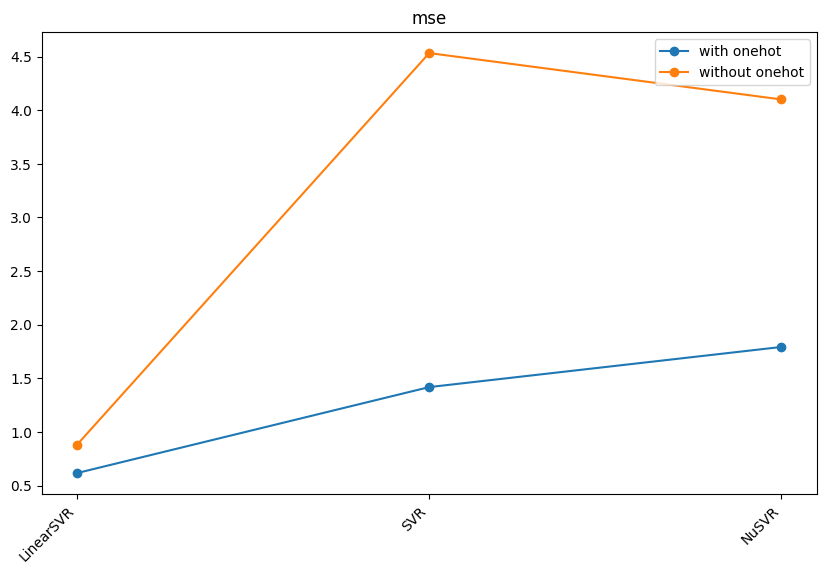
\includegraphics[width=6cm]{svm_mse.png} 
		\caption{One-Hot or not} 
		\label{Fig.svm_mse} 
		\end{figure}
		\begin{figure}[H]
		\centering
		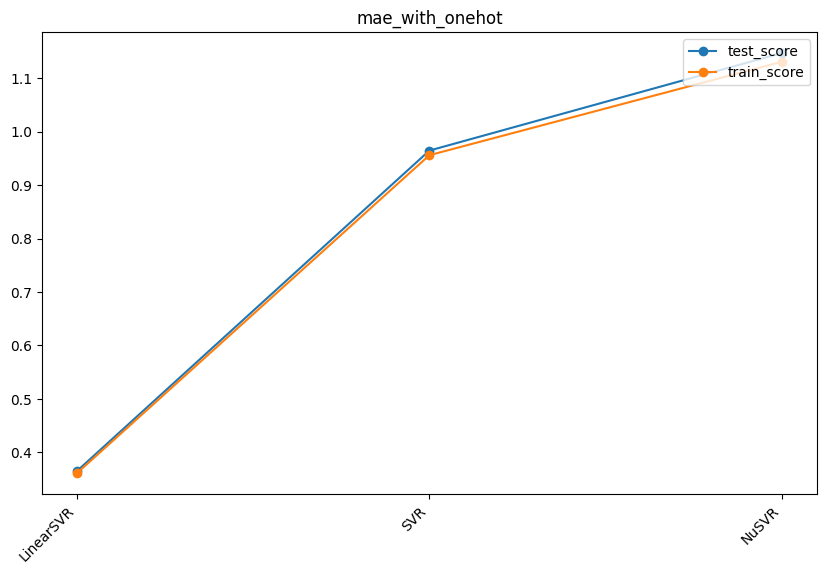
\includegraphics[width=6cm]{svm_loss.png} 
		\caption{Train vs Test} 
		\label{Fig.svm_loss} 
		\end{figure}
	We observe that in SVM, the dataset subjected to one-hot encoding demonstrates superior performance. Additionally, Linear SVR outperforms the general SVR, which, in turn, surpasses nuSVR. We hypothesize that the dataset subjected to one-hot encoding facilitates a better identification of the cutting plane.

As for the reason why Linear SVR outperforms the two kernel SVRs, we speculate that it is due to the setting of the maximum iteration count. We found that the training loss and test loss consistently remain identical, indicating that the function has not yet found an optimal cutting plane. Therefore, owing to the quicker convergence of Linear SVR, it exhibits superior performance.
	\subsection{Traditional models}
		\begin{figure}[H]
		\centering
		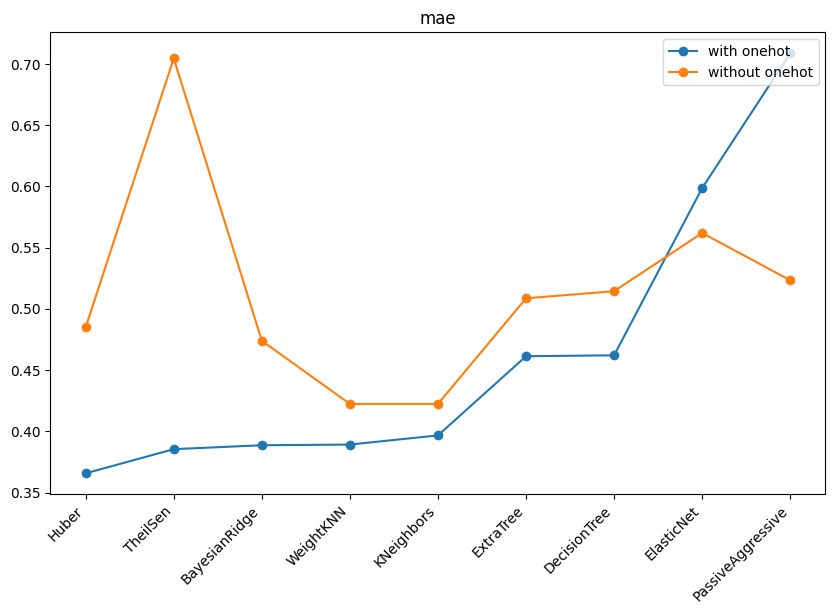
\includegraphics[width=6cm]{tradition_mae.png} 
		\caption{One-Hot or not} 
		\label{Fig.tradition_mae} 
		\end{figure}
		\begin{figure}[H]
		\centering
		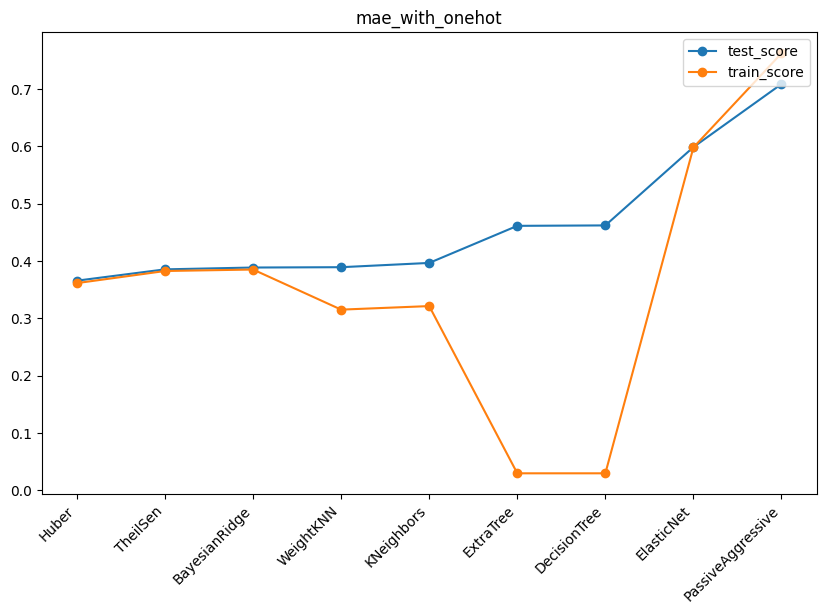
\includegraphics[width=6cm]{tradition_loss.png} 
		\caption{Train vs Test} 
		\label{Fig.svm_loss} 
		\end{figure}
When viewed as a whole, we can observe that most models perform better on datasets that have undergone one-hot encoding. Huber regression demonstrates stronger performance, indicating that the poor performance of linear regression may be attributed to the absence of regularization, given that Huber regression is essentially linear regression with the loss function replaced by the Huber function.

From the charts, it is evident that Weighted KNN outperforms regular KNN, suggesting that assigning weights to features before applying KNN contributes to loss reduction.

Considering the superior generalization capabilities of decision tree-type models compared to linear regression models in handling interactions among high-dimensional features, we hypothesize that decision tree and Extremely tree models exhibit significant overfitting, as also evident in the loss graphs.

Passive regression adjusts significantly for erroneous instances. Before one-hot encoding, adjustments are not pronounced due to less apparent errors. However, after one-hot encoding, with an increase in different class categories, errors are amplified, resulting in an abnormal increase in loss. The prowess of Passive Regression is notable before one-hot encoding but diminishes thereafter.

For the Teilsen model, the loss is exceptionally high before one-hot encoding. We speculate that this might be due to the presence of a substantial amount of similar data with considerable variations in the target variable, surpassing Teilsen's tolerance threshold and leading to subpar performance.
	\subsection{Ensemble Models}
		\begin{figure}[H]
		\centering
		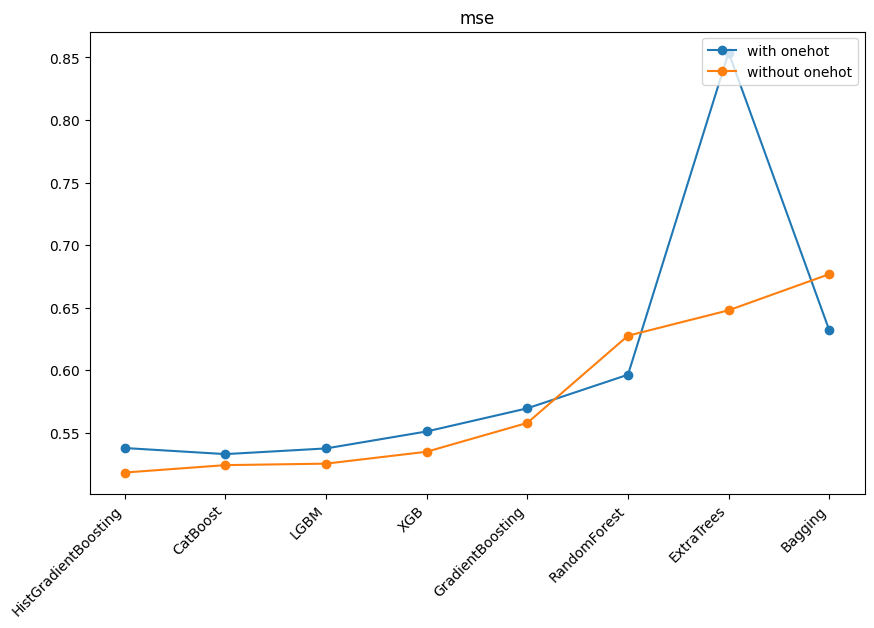
\includegraphics[width=6cm]{ensemble_mse.png} 
		\caption{One-Hot or not} 
		\label{Fig.ensemble_mse} 
		\end{figure}
		\begin{figure}[H]
		\centering
		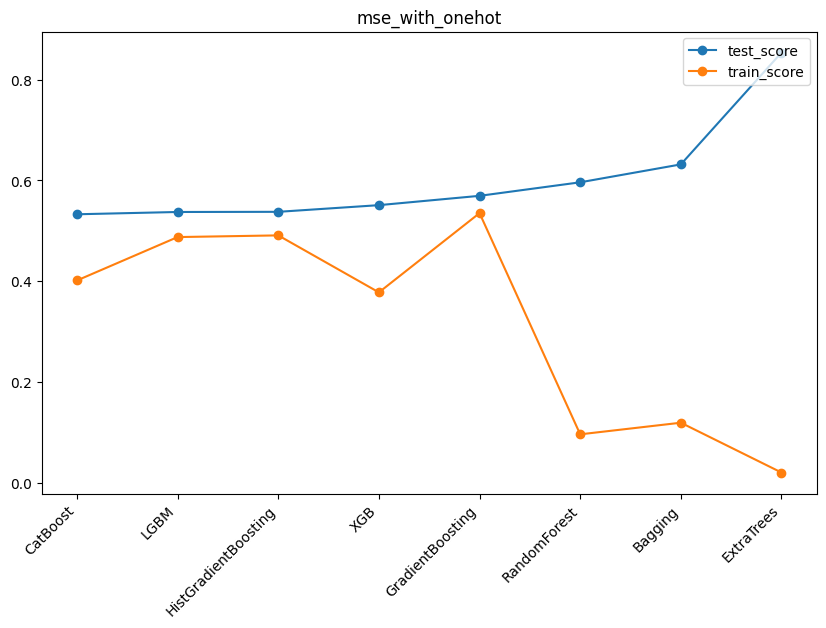
\includegraphics[width=6cm]{ensemble_mse_loss_wi.png} 
		\caption{Train vs Test} 
		\label{Fig.svm_loss} 
		\end{figure}
		\begin{figure}[H]
		\centering
		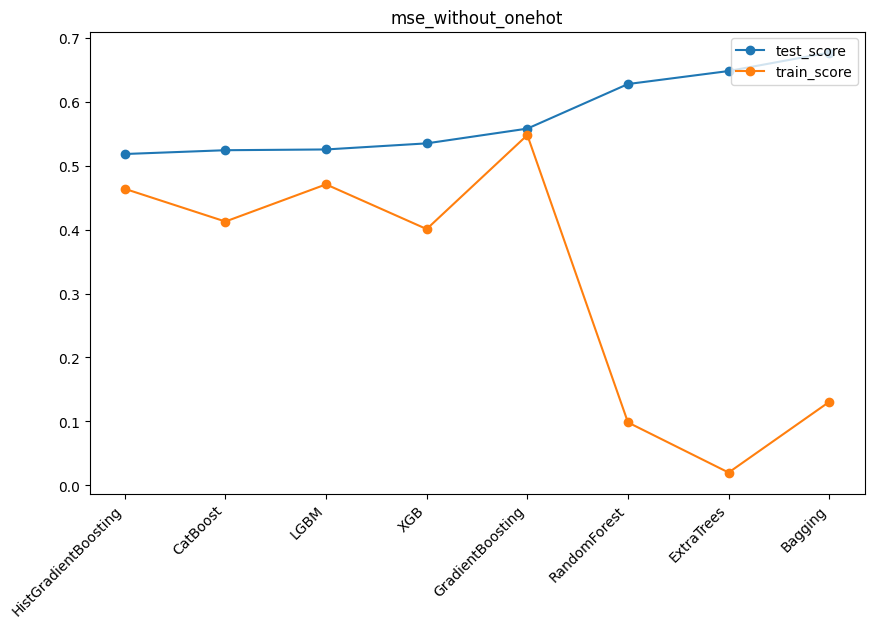
\includegraphics[width=6cm]{ensemble_mse_loss_wh.png} 
		\caption{Train vs Test} 
		\label{Fig.svm_loss} 
		\end{figure}
Due to the subpar performance of Adaboost, we temporarily removed it from the charts to emphasize the differences in other models. We speculate that fitting solely based on residual errors is not effective in capturing the data, and gradient-based methods are still necessary. From the graphs, it is evident that, apart from Random Forest and Bagging Model, Ensemble Models outperform when dealing with our dataset compared to processing one-hot encoded data. We hypothesize that the high dimensionality of 244 after expansion results in too many ways to split, causing overfitting in Decision Tree-based Ensemble Models. The loss chart indicates noticeable overfitting in one-hot processed CatBoost and XGBoost. As for why LightGBM hasn't exhibited clear overfitting, we attribute it to the structure of its leaf-wise trees. However, we believe that even increasing the number of LightGBM trees won't effectively fit the one-hot encoded dataset due to the combination of high dimensionality and insufficient data.

Regarding Extremely Trees, the explosive performance after one-hot encoding is evident. It can be inferred that this algorithm, which highly randomly selects features for data splitting, performs poorly in high-dimensional sparse data and easily leads to overfitting. The loss chart also highlights that Extremely Trees exhibits the most severe overfitting.
	\subsection{Neural Network}

\begin{table}[h]
\centering
\sisetup{
	tight-spacing=true,
    table-format=2.3e+2,
    scientific-notation=true,
    exponent-product=\times,
    separate-uncertainty=true,
    round-precision=3,
    round-mode=figures
}
\caption{Neural Network MAE}
\begin{tabularx}{\linewidth}{l *{2}{S}}
\toprule
\textbf{Name} & {\textbf{Test Loss}} & {\textbf{Train Loss}} \\
\midrule
MLP & 0.5866 & 0.5824 \\
MLP one-hot & 0.2900 & 0.2850 \\
MLP embedding & 0.3482 & 0.34131 \\
\bottomrule
\end{tabularx}

\caption{Neural Network MSE}
\begin{tabularx}{\linewidth}{l *{2}{S}}
\toprule
\textbf{Name} & {\textbf{Test Loss}} & {\textbf{Train Loss}} \\
\midrule
MLP & 0.3947 & 0.3927 \\
MLP one-hot & 0.3210 & 0.3210 \\
MLP embedding & 0.2074 & 0.2025 \\
\bottomrule
\end{tabularx}
\end{table}

In the context of this study, the neural network employed was a meticulously constructed model, featuring a multilayer perceptron with 244 input nodes, 128 hidden nodes, and 1 output node, serving as the baseline architecture. While variations in parameters may exist between the versions with and without one-hot encoding or embeddings, we exerted diligent efforts to fine-tune these models to ensure a consistent set of overall parameters.

The outcomes of our model distinctly illustrate the superior performance achieved when utilizing one-hot encoding or embeddings in comparison to their non-processed counterpart, underscoring the crucial role of preprocessing methodologies. Within the dataset, characterized by a substantial volume of akin prediction data, the neural network adeptly captures and models these intricacies, resulting in remarkably low mean square error (MSE) and mean absolute error (MAE) values. Further exploration of this phenomenon is warranted and will be expounded upon in the concluding sections.

Observations pertaining to the modest discrepancy between training and testing losses suggest that the model exhibits potential for further fitting. At present, there is a lack of discernible overfitting or underfitting issues, indicating a robust and well-generalized model.

\section{Conclusion}
\begin{figure}[H]
\centering
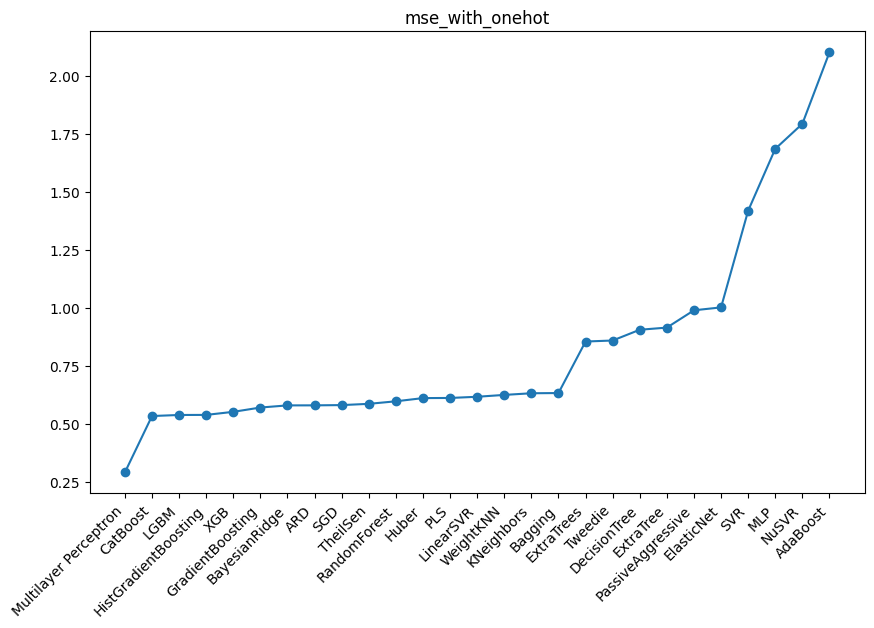
\includegraphics[width=6cm]{mse_with_onehot.png} 
\caption{MSE Overall} 
\label{Fig.mse_with_onehot} 
\end{figure}
In the models we trained, the rankings of each model reflect their performance in handling the respective tasks. These models encompass various directions, including deep learning, gradient boosting machines, ensemble models, linear regression, etc. Although each model has its unique features and advantages, their performances from best to worst can be visually observed in the charts. The following is a summary of the classification and relevant algorithms of all models, discussed in terms of model performance:

\begin{enumerate}[label= \textbf{\arabic*.}, left=0pt, itemsep=4pt]

\item \textbf{Deep Learning Models:}
    \begin{itemize}
        \item \textbf{Multilayer Perceptron (MLPRegressor):} A multilayer perceptron is a deep learning model based on neural networks, featuring multiple hidden layers and non-linear activation functions. It excels in many tasks, particularly when dealing with large datasets and complex patterns.
    \end{itemize}

\item \textbf{Gradient Boosting Machine Models:}
    \begin{itemize}
        \item \textbf{CatBoostRegressor, LGBMRegressor, HistGradientBoostingRegressor, XGBRegressor, GradientBoostingRegressor:} These models belong to the gradient boosting machine (GBM) category, typically suitable for regression problems. They progressively enhance model performance through ensemble methods, optimizing predictive outcomes.
    \end{itemize}

\item \textbf{Ensemble Models:}
    \begin{itemize}
        \item \textbf{RandomForestRegressor, BaggingRegressor, ExtraTreesRegressor:} These models utilize ensemble learning approaches, improving performance by integrating predictions from multiple base models. Random forest, bagging, and extremely randomized trees employ different strategies.
    \end{itemize}

\item \textbf{Linear Regression Models:}
    \begin{itemize}
        \item \textbf{BayesianRidge, ARDRegression, SGDRegressor, TheilSenRegressor, LinearSVR, WeightKNN, LinearRegression, RANSACRegressor:} These models fall under the linear regression category, modeling the linear relationships between features, suitable for linear structures in data.
    \end{itemize}

\item \textbf{Other Regression Models:}
    \begin{itemize}
        \item \textbf{HuberRegressor, PLSRegression, TweedieRegressor, DecisionTreeRegressor, ExtraTreeRegressor, PassiveAggressiveRegressor, ElasticNet, SVR, NuSVR, AdaBoostRegressor:} These models encompass various other regression methods, covering different statistical and machine learning techniques.
    \end{itemize}

\end{enumerate}

In conclusion, these model rankings provide insights into the performance of different types of models and serve as a reference for selecting appropriate models. Deep learning models excel in handling complex patterns and large datasets, while gradient boosting machines and ensemble models significantly outperform in integrating predictions from multiple weak models. Linear regression models are suitable for simple linear structures, and other regression models offer a diverse set of choices to address different characteristics in the data. This comprehensive ranking and summary will provide practical reference points for further research and model optimization.

\newpage
\printbibliography[heading=bibintoc, title={References}]
\nocite{*}

\appendix
\section{Dataset}
The dataset under consideration originates from the Family Income and Expenditure Statistics provided by the Directorate-General of Budget, Accounting, and Statistics, Executive Yuan. This statistical compilation encompasses a variety of indicators, including the Disposable Income Gap, Average Household Income and Expenditure, Family Consumption Expenditure Structure, Household Equipment Ownership Rate, and Homeownership Rate. The data is disseminated through the Local Statistics Promotion Center of the Directorate-General of Budget, Accounting, and Statistics, and compiled by the Family Income and Expenditure Section. For inquiries, the contact details include a phone number at 049-2394069 ext. 2345 and an email address at abigail@dgbas.gov.tw.

The dataset is available in multiple formats, including written publications such as press releases and the "Family Income and Expenditure Survey Report." Additionally, electronic versions of the data can be accessed online through the official website of the Directorate-General of Budget, Accounting, and Statistics (\url{https://www.stat.gov.tw/np.asp?ctNode=509&mp=4}). Notably, the dataset covers the entire Taiwan region, focusing on individuals with Republic of China citizenship residing in the area, forming households engaged in common economic activities. The statistical data is based on the calendar year, with the survey period spanning from January 1st to December 31st.

To ensure data quality, the Family Income and Expenditure Survey employs a two-stage stratified random sampling method. Cross-verification mechanisms are implemented to address extreme values and verify the accuracy of income and expenditure items. The dataset is released annually, and the information is typically made available eight months after the conclusion of the statistical standard time. The dataset has a long history, dating back to 1953 when the survey began. Over the years, various government agencies have been involved in its execution, adapting to changes in administrative divisions.

The dataset provides valuable insights into the economic landscape of Taiwan, covering aspects such as income distribution, household expenditures, and ownership rates of various amenities. Researchers and policymakers can leverage this comprehensive dataset to analyze trends, assess economic disparities, and make informed decisions. It serves as a foundational resource for understanding the financial dynamics within Taiwanese households.
\section{Dataset Column Description}
	\subsubsection{Relationship with the Head of Economic Household (Title: REL)}
		
\begin{itemize}
    \item \textbf{Self:} The individual recorded in the data is the head of the economic household.
    \item \textbf{Spouse:} The individual recorded in the data is the spouse of the head of the economic household.
    \item \textbf{Children (including adopted children):} The individual recorded in the data is the child of the head of the economic household, including adopted children.
    \item \textbf{Grandchildren (including internal and external grandchildren):} The individual recorded in the data is the grandchild of the head of the economic household, including internal and external grandchildren.
    \item \textbf{Head of Household's Grandchildren:} The individual recorded in the data is a grandchild of the head of the economic household.
    \item \textbf{Parents (including step-parents and foster parents):} The individual recorded in the data is the parent of the head of the economic household, including step-parents and foster parents.
    \item \textbf{Grandparents (including internal and external grandparents):} The individual recorded in the data is the grandparent of the head of the economic household, including internal and external grandparents.
    \item \textbf{Head of Household's Grandparents and Other Ancestors:} The individual recorded in the data is the grandparents and other ancestors of the head of the economic household.
    \item \textbf{Head of Household's Uncles and Aunts:} The individual recorded in the data is the uncles and aunts of the head of the economic household.
    \item \textbf{Siblings:} The individual recorded in the data is a sibling of the head of the economic household.
    \item \textbf{Children's Spouses:} The individual recorded in the data is the spouse of the children of the head of the economic household.
    \item \textbf{Head of Household's Nephews, Nieces, and Their Spouses:} The individual recorded in the data is the nephews, nieces, and their spouses of the head of the economic household.
    \item \textbf{Grandchildren's Spouses:} The individual recorded in the data is the spouse of the grandchildren of the head of the economic household.
    \item \textbf{Siblings' Spouses:} The individual recorded in the data is the spouse of the siblings of the head of the economic household.
    \item \textbf{Parents-in-law:} The individual recorded in the data is the parent of the spouse of the head of the economic household.
    \item \textbf{Siblings-in-law:} The individual recorded in the data is the sibling of the spouse of the head of the economic household.
    \item \textbf{Other Relatives:} The individual recorded in the data is another relative of the head of the economic household.
    \item \textbf{Other:} The individual recorded in the data has another relationship with the head of the economic household.
    \item \textbf{Relatives' Friends:} The individual recorded in the data is a friend of the relatives of the head of the economic household.
    \item \textbf{Long-term Worker (with common economic activities):} The individual recorded in the data is a long-term worker with common economic activities with the head of the economic household.
\end{itemize}
	\subsubsection{Gender Relationship with the Head of Economic Household (Title: SEX)}

\begin{itemize}
    \item \textbf{Male:} The individual recorded in the data is male.
    \item \textbf{Female:} The individual recorded in the data is female.
\end{itemize}

	\subsubsection{Educational Relationship with the Head of Economic Household (Title: EDU)}

\begin{itemize}
    \item \textbf{Illiterate:} The individual recorded in the data is illiterate.
    \item \textbf{Self-Taught:} The individual recorded in the data has acquired education through self-study.
    \item \textbf{Tutoring, Self-Taught, or Private Tutoring:} The individual recorded in the data has received education through tutoring, self-study, or private tutoring.
    \item \textbf{Elementary School:} The individual recorded in the data has completed elementary school education.
    \item \textbf{Junior High School (Junior Vocational):} The individual recorded in the data has completed junior high school or junior vocational education.
    \item \textbf{Junior Vocational:} The individual recorded in the data has completed junior vocational education.
    \item \textbf{Junior High School:} The individual recorded in the data has completed junior high school education.
    \item \textbf{High School:} The individual recorded in the data has completed high school education.
    \item \textbf{Vocational High School:} The individual recorded in the data has completed vocational high school education.
    \item \textbf{Junior College (Before the Three-Year Division with Vocational High School):} The individual recorded in the data has completed junior college education, which includes the three-year division with vocational high school.
    \item \textbf{University:} The individual recorded in the data has completed university education.
    \item \textbf{Graduate School:} The individual recorded in the data has completed graduate school education.
    \item \textbf{Master's Degree:} The individual recorded in the data has obtained a master's degree.
    \item \textbf{Doctorate:} The individual recorded in the data has obtained a doctorate.
\end{itemize}

	\subsubsection{Occupational Relationship with Industry (Title: IND)}

\begin{itemize}
    \item \textbf{No Occupation (Including Head of Economic Household with No Occupation):} The individual recorded in the data is not employed, including the head of the economic household with no occupation.
    \item \textbf{Agriculture, Forestry, Fishing, Hunting:} The individual recorded in the data is engaged in agriculture, forestry, fishing, or hunting.
    \item \textbf{Farm or Livestock Industry:} The individual recorded in the data is engaged in the farm or livestock industry.
    \item \textbf{Farm, Livestock, Hunting:} The individual recorded in the data is engaged in farm, livestock, or hunting activities.
    \item \textbf{Forestry and Logging:} The individual recorded in the data is engaged in forestry and logging.
    \item \textbf{Fishing Industry:} The individual recorded in the data is engaged in the fishing industry.
    \item \textbf{Mining and Quarrying:} The individual recorded in the data is engaged in mining and quarrying activities.
    \item \textbf{Manufacturing Industry:} The individual recorded in the data is engaged in the manufacturing industry.
    \item \textbf{Water, Electricity, Gas Industry:} The individual recorded in the data is engaged in the water, electricity, and gas industry.
    \item \textbf{Electricity and Gas Supply Industry:} The individual recorded in the data is engaged in the electricity and gas supply industry.
    \item \textbf{Water Supply and Pollution Control Industry:} The individual recorded in the data is engaged in the water supply and pollution control industry.
    \item \textbf{Construction Industry:} The individual recorded in the data is engaged in the construction industry.
    \item \textbf{Wholesale, Retail, and Restaurant Industry:} The individual recorded in the data is engaged in the wholesale, retail, and restaurant industry.
    \item \textbf{Wholesale and Retail Industry:} The individual recorded in the data is engaged in the wholesale and retail industry.
    \item \textbf{Accommodation and Restaurant Industry:} The individual recorded in the data is engaged in the accommodation and restaurant industry.
    \item \textbf{Commerce:} The individual recorded in the data is engaged in commerce.
    \item \textbf{Transportation, Warehousing, and Communication Industry:} The individual recorded in the data is engaged in the transportation, warehousing, and communication industry.
    \item \textbf{Transportation and Warehousing Industry:} The individual recorded in the data is engaged in the transportation and warehousing industry.
    \item \textbf{Information and Communication Industry:} The individual recorded in the data is engaged in the information and communication industry.
    \item \textbf{Finance, Insurance, Real Estate:} The individual recorded in the data is engaged in finance, insurance, and real estate.
    \item \textbf{Finance and Insurance Industry:} The individual recorded in the data is engaged in the finance and insurance industry.
    \item \textbf{Real Estate and Leasing Industry:} The individual recorded in the data is engaged in the real estate and leasing industry.
    \item \textbf{Real Estate Industry:} The individual recorded in the data is engaged in the real estate industry.
    \item \textbf{Industrial and Commercial Service Industry:} The individual recorded in the data is engaged in industrial and commercial service industry.
    \item \textbf{Social Service and Personal Service Industry:} The individual recorded in the data is engaged in social service and personal service industry.
    \item \textbf{Professional, Scientific, and Technical Service Industry:} The individual recorded in the data is engaged in professional, scientific, and technical service industry.
    \item \textbf{Support Service Industry:} The individual recorded in the data is engaged in support service industry.
    \item \textbf{Education Service Industry:} The individual recorded in the data is engaged in education service industry.
    \item \textbf{Healthcare and Social Welfare Service Industry:} The individual recorded in the data is engaged in healthcare and social welfare service industry.
    \item \textbf{Healthcare and Social Work Service Industry:} The individual recorded in the data is engaged in healthcare and social work service industry.
    \item \textbf{Culture, Sports, and Leisure Service Industry:} The individual recorded in the data is engaged in culture, sports, and leisure service industry.
    \item \textbf{Art, Entertainment, and Leisure Service Industry:} The individual recorded in the data is engaged in art, entertainment, and leisure service industry.
    \item \textbf{Other Service Industry:} The individual recorded in the data is engaged in other service industry.
    \item \textbf{Public Administration Industry:} The individual recorded in the data is engaged in public administration industry.
    \item \textbf{Public Administration and National Defense; Mandatory Social Security:} The individual recorded in the data is engaged in public administration and national defense, including mandatory social security.
    \item \textbf{Other Unclassifiable Industry:} The individual recorded in the data is engaged in an industry that cannot be classified under the specified categories.
\end{itemize}

	\subsubsection{Occupation Type (Title: OCC)}

\begin{itemize}
    \item \textbf{No Occupation (Including Head of Economic Household with No Occupation):} The individual recorded in the data is not employed, including the head of the economic household with no occupation.
    \item \textbf{Public Representative, Administrative Executive, Corporate Executive, and Manager:} The individual recorded in the data holds a position as a public representative, administrative executive, corporate executive, or manager.
    \item \textbf{Public Representative, Executive, and Manager:} The individual recorded in the data holds a position as a public representative, executive, or manager.
    \item \textbf{Professional:} The individual recorded in the data is a professional.
    \item \textbf{Technician and Assistant Professional:} The individual recorded in the data is a technician or assistant professional.
    \item \textbf{Clerical Workers:} The individual recorded in the data is a clerical worker.
    \item \textbf{Clerical Support Staff:} The individual recorded in the data is a clerical support staff.
    \item \textbf{Service Workers and Salespersons:} The individual recorded in the data is a service worker or salesperson.
    \item \textbf{Service and Sales Workers:} The individual recorded in the data is a service and sales worker.
    \item \textbf{Specialized, Technical, and Related Personnel:} The individual recorded in the data is specialized, technical, or related personnel.
    \item \textbf{Administrative and Executive Personnel:} The individual recorded in the data is administrative and executive personnel.
    \item \textbf{Supervisory and Clerical Staff:} The individual recorded in the data is supervisory and clerical staff.
    \item \textbf{Buying and Selling Workers:} The individual recorded in the data is involved in buying and selling.
    \item \textbf{Service Workers:} The individual recorded in the data is a service worker.
    \item \textbf{Agriculture, Forestry, Fishing, and Hunting Workers:} The individual recorded in the data is a worker engaged in agriculture, forestry, fishing, or hunting.
    \item \textbf{Agricultural, Livestock, and Related Workers:} The individual recorded in the data is a worker engaged in agricultural, livestock, or related activities.
    \item \textbf{Agriculture, Livestock, Hunting, and Related Workers:} The individual recorded in the data is a worker engaged in agriculture, livestock, hunting, or related activities.
    \item \textbf{Forestry and Related Workers:} The individual recorded in the data is a worker engaged in forestry and related activities.
    \item \textbf{Forestry Production Personnel:} The individual recorded in the data is forestry production personnel.
    \item \textbf{Fishing and Related Workers:} The individual recorded in the data is a worker engaged in fishing and related activities.
    \item \textbf{Fishing Production Personnel:} The individual recorded in the data is fishing production personnel.
    \item \textbf{Technical Workers and Related Personnel:} The individual recorded in the data is a technical worker or related personnel.
    \item \textbf{Artisan and Related Workers:} The individual recorded in the data is an artisan or related worker.
    \item \textbf{Machinery Operation and Assembly Workers:} The individual recorded in the data is a machinery operation and assembly worker.
    \item \textbf{Machinery Operation and Assembly Personnel:} The individual recorded in the data is machinery operation and assembly personnel.
    \item \textbf{Non-technical and Manual Workers:} The individual recorded in the data is a non-technical and manual worker.
    \item \textbf{Grassroots Technical Workers and Laborers:} The individual recorded in the data is a grassroots technical worker and laborer.
    \item \textbf{Production and Related Workers:} The individual recorded in the data is a production and related worker.
    \item \textbf{Transportation Equipment Operators:} The individual recorded in the data is a transportation equipment operator.
    \item \textbf{Apprentices and Other Manual Workers:} The individual recorded in the data is an apprentice or other manual worker.
    \item \textbf{Manual Workers:} The individual recorded in the data is a manual worker.
    \item \textbf{Active Military Personnel:} The individual recorded in the data is an active military personnel.
    \item \textbf{Occupations Unable to be Classified:} The individual recorded in the data is engaged in an occupation that cannot be classified under specified categories.
    \item \textbf{Teacher:} The individual recorded in the data is a teacher.
\end{itemize}

	\subsubsection{Employment Status (Title: WKCLASS)}

\begin{itemize}
    \item \textbf{Employer:} The individual recorded in the data is an employer.
    \item \textbf{Employee (Hired):} The individual recorded in the data is an employee who is hired by an employer.
    \item \textbf{Self-employed:} The individual recorded in the data is self-employed.
    \item \textbf{Unpaid Family Worker:} The individual recorded in the data is an unpaid family worker.
    \item \textbf{Unemployed:} The individual recorded in the data is unemployed.
    \item \textbf{Child (Under 7 Years Old):} The individual recorded in the data is a child under the age of 7.
    \item \textbf{Child (Under 6 Years Old):} The individual recorded in the data is a child under the age of 6.
    \item \textbf{Student (Including those attending supplementary classes):} The individual recorded in the data is a student, including those attending supplementary classes.
    \item \textbf{Homemaker (Husband/Wife):} The individual recorded in the data is a homemaker (husband or wife).
    \item \textbf{Other (Including children under 7 years old, first-year elementary school students, children aged 7-14 not attending school, and those without a willingness to work):} The individual recorded in the data falls under other categories, including children under 7 years old, first-year elementary school students, children aged 7-14 not attending school, and those without a willingness to work.
    \item \textbf{Other (Including children aged 7-14 not attending school and those without a willingness to work):} The individual recorded in the data falls under other categories, including children aged 7-14 not attending school and those without a willingness to work.
    \item \textbf{Other (Including children aged 7-14 not attending school, individuals aged 65 and above, and those who are physically or mentally challenged):} The individual recorded in the data falls under other categories, including children aged 7-14 not attending school, individuals aged 65 and above, and those who are physically or mentally challenged.
    \item \textbf{Other (Including children aged 6-14 not attending school, individuals aged 65 and above, and those who are physically or mentally challenged):} The individual recorded in the data falls under other categories, including children aged 6-14 not attending school, individuals aged 65 and above, and those who are physically or mentally challenged.
\end{itemize}

	\subsubsection{Employment Status Type (Title: WORK)}

\begin{itemize}
    \item \textbf{Employed:} Individuals recorded in the data are currently employed.
    \item \textbf{Not Employed:} Individuals recorded in the data are not currently employed.
\end{itemize}

	\subsubsection{Income Recipient Type (Title: IMR)}

\begin{itemize}
    \item \textbf{Income Recipient:} Individuals in this category are identified as recipients of income.
    \item \textbf{Non-Income Recipient:} Individuals in this category are not recipients of income.
\end{itemize}

	\subsubsection{Workplace (Title: WORKPLACE)}

\begin{itemize}
    \item \textbf{Taipei County}
    \item \textbf{Yilan County}
    \item \textbf{Taoyuan County}
    \item \textbf{Hsinchu County}
    \item \textbf{Miaoli County}
    \item \textbf{Taipei City}
    \item \textbf{Taipei City}
    \item \textbf{Changhua County}
    \item \textbf{Nantou County}
    \item \textbf{Yunlin County}
    \item \textbf{Chiayi County}
    \item \textbf{Tainan County}
    \item \textbf{Kaohsiung County}
    \item \textbf{Pingtung County}
    \item \textbf{Taitung County}
    \item \textbf{Hualien County}
    \item \textbf{Penghu County}
    \item \textbf{Keelung City}
    \item \textbf{Hsinchu City}
    \item \textbf{Taipei City}
    \item \textbf{Kaohsiung City}
    \item \textbf{New Taipei City}
    \item \textbf{Taipei City}
    \item \textbf{Taipei City}
    \item \textbf{Taipei City}
    \item \textbf{Kinmen and Matsu Region}
    \item \textbf{Lienchiang County}
    \item \textbf{Kinmen County}
    \item \textbf{Abroad (including Mainland China)}
    \item \textbf{Previously received one-time employer-provided retirement pension}
    \item \textbf{Military retirement (soldiers)}
    \item \textbf{Civilian retirement (including police monthly retirement, labor retirement pension monthly)}
\end{itemize}

		\subsubsection{Marital Status (Title: MRG)}

\begin{itemize}
    \item \textbf{Single:} Individuals who have never been married.
    
    \item \textbf{Spouse is a household member:} Individuals who are currently married, and their spouse is a member of the same household.
    
    \item \textbf{Spouse is a non-household member:} Individuals who are currently married, but their spouse resides in a different household.
    
    \item \textbf{Cohabiting:} Individuals who live together in a relationship without being legally married.
    
    \item \textbf{Divorced:} Individuals who have legally ended their marriage through divorce.
    
    \item \textbf{Separated:} Individuals who are currently living apart from their spouse but have not finalized a legal divorce.
    
    \item \textbf{Widowed:} Individuals who have lost their spouse due to death.
\end{itemize}


\end{document}
